% Anonymous IJDC edition, generated from the journal revision sources.
\documentclass[iicol,pdflatex,sn-basic,Numbered]{sn-jnl}
\usepackage{graphicx}
\usepackage{amsmath,amssymb,amsfonts}
\usepackage{booktabs,siunitx,xcolor}
\usepackage[title]{appendix}
\hypersetup{pdftitle={Complementary-Filtered Residual World Models for Multistep Prediction of Nonlinear Controlled Dynamics},pdfauthor={},pdfsubject={},pdfkeywords={}}
\newcommand{\method}{CFR-WM}
\newcommand{\vect}[1]{\mathbf{#1}}
% Generated only from locked results/confirmatory_analysis artifacts.
\newcommand{\PrimaryBaseline}{PGNN-style}
\newcommand{\PrimaryDifference}{-0.0098}
\newcommand{\PrimaryCILow}{-0.0121}
\newcommand{\PrimaryCIHigh}{-0.0075}
\newcommand{\PrimaryImprovement}{8.97}
\newcommand{\PrimaryRelativeCILow}{6.88}
\newcommand{\PrimaryRelativeCIHigh}{10.95}
\newcommand{\PrimaryPValue}{0.00391}
\newcommand{\PrimaryDecision}{supported}
\newcommand{\PrimaryInterpretation}{supports the prespecified practical-gain claim}
\newcommand{\RobustnessDecision}{not supported}
\newcommand{\RobustnessInterpretation}{does not support the gated robustness claim}
\newcommand{\CorruptImprovement}{12.05}
\newcommand{\CorruptRelativeCILow}{10.51}
\newcommand{\CorruptRelativeCIHigh}{13.49}
\newcommand{\CorruptPValue}{0.00391}
\newcommand{\CleanImprovement}{-13.08}
\newcommand{\CleanRelativeCILow}{-20.60}
\newcommand{\CleanRelativeCIHigh}{-5.67}
\newcommand{\CleanPValue}{0.95703}
\newcommand{\CFRNRMSE}{0.0998}
\newcommand{\PGNNNRMSE}{0.1096}
\newcommand{\BestMethod}{CFR-WM}
\newcommand{\BestNRMSE}{0.0998}
\newcommand{\BestGain}{0.50}
\newcommand{\OneStepImprovement}{59.38}
\newcommand{\OneStepRelativeCILow}{48.88}
\newcommand{\OneStepRelativeCIHigh}{68.88}
\newcommand{\OneStepHolmP}{0.03906}
\newcommand{\CellsWorseTen}{3}
\newcommand{\CartpoleCleanChange}{+47.3}
\newcommand{\VanDerPolCleanChange}{+19.4}
\newcommand{\DuffingCleanChange}{+24.4}
\newcommand{\IDCorruptFavoredCount}{5}
\newcommand{\IDCorruptCellCount}{5}
\newcommand{\IDCorruptLeastChange}{-13.3}
\newcommand{\IDCorruptMostChange}{-34.8}
\newcommand{\AllMetricsFinite}{yes}
\newcommand{\UniqueDataHashes}{40}
\newcommand{\ConfirmatoryRuns}{440}
\newcommand{\ConfirmatoryTrajectories}{126{,}720}
% Generated from verified saved external forecasts.
\newcommand{\ExternalTestFlights}{3}
\newcommand{\ExternalFinalSeeds}{5}
\newcommand{\ExternalLearnedParameters}{47000}
\newcommand{\ExternalForecastWindows}{387}
\newcommand{\ExternalCFRCombinedShortNRMSEMean}{0.401}
\newcommand{\ExternalCFRCombinedShortNRMSESD}{0.011}
\newcommand{\ExternalCFRCombinedShortPositionMean}{0.058}
\newcommand{\ExternalCFRCombinedShortPositionSD}{0.002}
\newcommand{\ExternalCFRCombinedShortVelocityMean}{0.133}
\newcommand{\ExternalCFRCombinedShortVelocitySD}{0.002}
\newcommand{\ExternalCFRCombinedLongNRMSEMean}{0.540}
\newcommand{\ExternalCFRCombinedLongNRMSESD}{0.014}
\newcommand{\ExternalCFRCombinedLongPositionMean}{0.094}
\newcommand{\ExternalCFRCombinedLongPositionSD}{0.004}
\newcommand{\ExternalCFRCombinedLongVelocityMean}{0.267}
\newcommand{\ExternalCFRCombinedLongVelocitySD}{0.014}
\newcommand{\ExternalCFRMissingShortNRMSEMean}{0.397}
\newcommand{\ExternalCFRMissingShortNRMSESD}{0.011}
\newcommand{\ExternalCFRMissingShortPositionMean}{0.038}
\newcommand{\ExternalCFRMissingShortPositionSD}{0.002}
\newcommand{\ExternalCFRMissingShortVelocityMean}{0.116}
\newcommand{\ExternalCFRMissingShortVelocitySD}{0.002}
\newcommand{\ExternalCFRMissingLongNRMSEMean}{0.537}
\newcommand{\ExternalCFRMissingLongNRMSESD}{0.014}
\newcommand{\ExternalCFRMissingLongPositionMean}{0.081}
\newcommand{\ExternalCFRMissingLongPositionSD}{0.005}
\newcommand{\ExternalCFRMissingLongVelocityMean}{0.259}
\newcommand{\ExternalCFRMissingLongVelocitySD}{0.014}
\newcommand{\ExternalCFRNoiseShortNRMSEMean}{0.393}
\newcommand{\ExternalCFRNoiseShortNRMSESD}{0.012}
\newcommand{\ExternalCFRNoiseShortPositionMean}{0.058}
\newcommand{\ExternalCFRNoiseShortPositionSD}{0.002}
\newcommand{\ExternalCFRNoiseShortVelocityMean}{0.129}
\newcommand{\ExternalCFRNoiseShortVelocitySD}{0.003}
\newcommand{\ExternalCFRNoiseLongNRMSEMean}{0.532}
\newcommand{\ExternalCFRNoiseLongNRMSESD}{0.017}
\newcommand{\ExternalCFRNoiseLongPositionMean}{0.091}
\newcommand{\ExternalCFRNoiseLongPositionSD}{0.003}
\newcommand{\ExternalCFRNoiseLongVelocityMean}{0.257}
\newcommand{\ExternalCFRNoiseLongVelocitySD}{0.014}
\newcommand{\ExternalCFRRecordedShortNRMSEMean}{0.389}
\newcommand{\ExternalCFRRecordedShortNRMSESD}{0.012}
\newcommand{\ExternalCFRRecordedShortPositionMean}{0.037}
\newcommand{\ExternalCFRRecordedShortPositionSD}{0.002}
\newcommand{\ExternalCFRRecordedShortVelocityMean}{0.113}
\newcommand{\ExternalCFRRecordedShortVelocitySD}{0.003}
\newcommand{\ExternalCFRRecordedLongNRMSEMean}{0.530}
\newcommand{\ExternalCFRRecordedLongNRMSESD}{0.016}
\newcommand{\ExternalCFRRecordedLongPositionMean}{0.078}
\newcommand{\ExternalCFRRecordedLongPositionSD}{0.003}
\newcommand{\ExternalCFRRecordedLongVelocityMean}{0.249}
\newcommand{\ExternalCFRRecordedLongVelocitySD}{0.015}
\newcommand{\ExternalNominalCombinedShortNRMSEMean}{0.506}
\newcommand{\ExternalNominalCombinedShortNRMSESD}{0.000}
\newcommand{\ExternalNominalCombinedShortPositionMean}{0.081}
\newcommand{\ExternalNominalCombinedShortPositionSD}{0.000}
\newcommand{\ExternalNominalCombinedShortVelocityMean}{0.160}
\newcommand{\ExternalNominalCombinedShortVelocitySD}{0.000}
\newcommand{\ExternalNominalCombinedLongNRMSEMean}{0.799}
\newcommand{\ExternalNominalCombinedLongNRMSESD}{0.000}
\newcommand{\ExternalNominalCombinedLongPositionMean}{0.105}
\newcommand{\ExternalNominalCombinedLongPositionSD}{0.000}
\newcommand{\ExternalNominalCombinedLongVelocityMean}{0.351}
\newcommand{\ExternalNominalCombinedLongVelocitySD}{0.000}
\newcommand{\ExternalNominalMissingShortNRMSEMean}{0.495}
\newcommand{\ExternalNominalMissingShortNRMSESD}{0.000}
\newcommand{\ExternalNominalMissingShortPositionMean}{0.025}
\newcommand{\ExternalNominalMissingShortPositionSD}{0.000}
\newcommand{\ExternalNominalMissingShortVelocityMean}{0.105}
\newcommand{\ExternalNominalMissingShortVelocitySD}{0.000}
\newcommand{\ExternalNominalMissingLongNRMSEMean}{0.792}
\newcommand{\ExternalNominalMissingLongNRMSESD}{0.000}
\newcommand{\ExternalNominalMissingLongPositionMean}{0.063}
\newcommand{\ExternalNominalMissingLongPositionSD}{0.000}
\newcommand{\ExternalNominalMissingLongVelocityMean}{0.320}
\newcommand{\ExternalNominalMissingLongVelocitySD}{0.000}
\newcommand{\ExternalNominalNoiseShortNRMSEMean}{0.498}
\newcommand{\ExternalNominalNoiseShortNRMSESD}{0.000}
\newcommand{\ExternalNominalNoiseShortPositionMean}{0.080}
\newcommand{\ExternalNominalNoiseShortPositionSD}{0.000}
\newcommand{\ExternalNominalNoiseShortVelocityMean}{0.154}
\newcommand{\ExternalNominalNoiseShortVelocitySD}{0.000}
\newcommand{\ExternalNominalNoiseLongNRMSEMean}{0.797}
\newcommand{\ExternalNominalNoiseLongNRMSESD}{0.000}
\newcommand{\ExternalNominalNoiseLongPositionMean}{0.103}
\newcommand{\ExternalNominalNoiseLongPositionSD}{0.000}
\newcommand{\ExternalNominalNoiseLongVelocityMean}{0.347}
\newcommand{\ExternalNominalNoiseLongVelocitySD}{0.000}
\newcommand{\ExternalNominalRecordedShortNRMSEMean}{0.488}
\newcommand{\ExternalNominalRecordedShortNRMSESD}{0.000}
\newcommand{\ExternalNominalRecordedShortPositionMean}{0.023}
\newcommand{\ExternalNominalRecordedShortPositionSD}{0.000}
\newcommand{\ExternalNominalRecordedShortVelocityMean}{0.102}
\newcommand{\ExternalNominalRecordedShortVelocitySD}{0.000}
\newcommand{\ExternalNominalRecordedLongNRMSEMean}{0.790}
\newcommand{\ExternalNominalRecordedLongNRMSESD}{0.000}
\newcommand{\ExternalNominalRecordedLongPositionMean}{0.063}
\newcommand{\ExternalNominalRecordedLongPositionSD}{0.000}
\newcommand{\ExternalNominalRecordedLongVelocityMean}{0.318}
\newcommand{\ExternalNominalRecordedLongVelocitySD}{0.000}
\newcommand{\ExternalRecurrentCombinedShortNRMSEMean}{0.405}
\newcommand{\ExternalRecurrentCombinedShortNRMSESD}{0.005}
\newcommand{\ExternalRecurrentCombinedShortPositionMean}{0.092}
\newcommand{\ExternalRecurrentCombinedShortPositionSD}{0.003}
\newcommand{\ExternalRecurrentCombinedShortVelocityMean}{0.175}
\newcommand{\ExternalRecurrentCombinedShortVelocitySD}{0.008}
\newcommand{\ExternalRecurrentCombinedLongNRMSEMean}{0.533}
\newcommand{\ExternalRecurrentCombinedLongNRMSESD}{0.006}
\newcommand{\ExternalRecurrentCombinedLongPositionMean}{0.126}
\newcommand{\ExternalRecurrentCombinedLongPositionSD}{0.006}
\newcommand{\ExternalRecurrentCombinedLongVelocityMean}{0.297}
\newcommand{\ExternalRecurrentCombinedLongVelocitySD}{0.020}
\newcommand{\ExternalRecurrentMissingShortNRMSEMean}{0.395}
\newcommand{\ExternalRecurrentMissingShortNRMSESD}{0.005}
\newcommand{\ExternalRecurrentMissingShortPositionMean}{0.051}
\newcommand{\ExternalRecurrentMissingShortPositionSD}{0.004}
\newcommand{\ExternalRecurrentMissingShortVelocityMean}{0.136}
\newcommand{\ExternalRecurrentMissingShortVelocitySD}{0.008}
\newcommand{\ExternalRecurrentMissingLongNRMSEMean}{0.526}
\newcommand{\ExternalRecurrentMissingLongNRMSESD}{0.007}
\newcommand{\ExternalRecurrentMissingLongPositionMean}{0.098}
\newcommand{\ExternalRecurrentMissingLongPositionSD}{0.007}
\newcommand{\ExternalRecurrentMissingLongVelocityMean}{0.277}
\newcommand{\ExternalRecurrentMissingLongVelocitySD}{0.019}
\newcommand{\ExternalRecurrentNoiseShortNRMSEMean}{0.398}
\newcommand{\ExternalRecurrentNoiseShortNRMSESD}{0.008}
\newcommand{\ExternalRecurrentNoiseShortPositionMean}{0.089}
\newcommand{\ExternalRecurrentNoiseShortPositionSD}{0.002}
\newcommand{\ExternalRecurrentNoiseShortVelocityMean}{0.164}
\newcommand{\ExternalRecurrentNoiseShortVelocitySD}{0.004}
\newcommand{\ExternalRecurrentNoiseLongNRMSEMean}{0.527}
\newcommand{\ExternalRecurrentNoiseLongNRMSESD}{0.006}
\newcommand{\ExternalRecurrentNoiseLongPositionMean}{0.120}
\newcommand{\ExternalRecurrentNoiseLongPositionSD}{0.004}
\newcommand{\ExternalRecurrentNoiseLongVelocityMean}{0.281}
\newcommand{\ExternalRecurrentNoiseLongVelocitySD}{0.016}
\newcommand{\ExternalRecurrentRecordedShortNRMSEMean}{0.388}
\newcommand{\ExternalRecurrentRecordedShortNRMSESD}{0.008}
\newcommand{\ExternalRecurrentRecordedShortPositionMean}{0.046}
\newcommand{\ExternalRecurrentRecordedShortPositionSD}{0.003}
\newcommand{\ExternalRecurrentRecordedShortVelocityMean}{0.128}
\newcommand{\ExternalRecurrentRecordedShortVelocitySD}{0.004}
\newcommand{\ExternalRecurrentRecordedLongNRMSEMean}{0.519}
\newcommand{\ExternalRecurrentRecordedLongNRMSESD}{0.006}
\newcommand{\ExternalRecurrentRecordedLongPositionMean}{0.091}
\newcommand{\ExternalRecurrentRecordedLongPositionSD}{0.005}
\newcommand{\ExternalRecurrentRecordedLongVelocityMean}{0.263}
\newcommand{\ExternalRecurrentRecordedLongVelocitySD}{0.016}
\newcommand{\ExternalUnfilteredCombinedShortNRMSEMean}{0.397}
\newcommand{\ExternalUnfilteredCombinedShortNRMSESD}{0.008}
\newcommand{\ExternalUnfilteredCombinedShortPositionMean}{0.092}
\newcommand{\ExternalUnfilteredCombinedShortPositionSD}{0.007}
\newcommand{\ExternalUnfilteredCombinedShortVelocityMean}{0.161}
\newcommand{\ExternalUnfilteredCombinedShortVelocitySD}{0.003}
\newcommand{\ExternalUnfilteredCombinedLongNRMSEMean}{0.534}
\newcommand{\ExternalUnfilteredCombinedLongNRMSESD}{0.019}
\newcommand{\ExternalUnfilteredCombinedLongPositionMean}{0.125}
\newcommand{\ExternalUnfilteredCombinedLongPositionSD}{0.017}
\newcommand{\ExternalUnfilteredCombinedLongVelocityMean}{0.268}
\newcommand{\ExternalUnfilteredCombinedLongVelocitySD}{0.009}
\newcommand{\ExternalUnfilteredMissingShortNRMSEMean}{0.386}
\newcommand{\ExternalUnfilteredMissingShortNRMSESD}{0.008}
\newcommand{\ExternalUnfilteredMissingShortPositionMean}{0.049}
\newcommand{\ExternalUnfilteredMissingShortPositionSD}{0.012}
\newcommand{\ExternalUnfilteredMissingShortVelocityMean}{0.115}
\newcommand{\ExternalUnfilteredMissingShortVelocitySD}{0.004}
\newcommand{\ExternalUnfilteredMissingLongNRMSEMean}{0.527}
\newcommand{\ExternalUnfilteredMissingLongNRMSESD}{0.020}
\newcommand{\ExternalUnfilteredMissingLongPositionMean}{0.095}
\newcommand{\ExternalUnfilteredMissingLongPositionSD}{0.022}
\newcommand{\ExternalUnfilteredMissingLongVelocityMean}{0.243}
\newcommand{\ExternalUnfilteredMissingLongVelocitySD}{0.009}
\newcommand{\ExternalUnfilteredNoiseShortNRMSEMean}{0.387}
\newcommand{\ExternalUnfilteredNoiseShortNRMSESD}{0.010}
\newcommand{\ExternalUnfilteredNoiseShortPositionMean}{0.087}
\newcommand{\ExternalUnfilteredNoiseShortPositionSD}{0.003}
\newcommand{\ExternalUnfilteredNoiseShortVelocityMean}{0.154}
\newcommand{\ExternalUnfilteredNoiseShortVelocitySD}{0.003}
\newcommand{\ExternalUnfilteredNoiseLongNRMSEMean}{0.523}
\newcommand{\ExternalUnfilteredNoiseLongNRMSESD}{0.018}
\newcommand{\ExternalUnfilteredNoiseLongPositionMean}{0.115}
\newcommand{\ExternalUnfilteredNoiseLongPositionSD}{0.007}
\newcommand{\ExternalUnfilteredNoiseLongVelocityMean}{0.258}
\newcommand{\ExternalUnfilteredNoiseLongVelocitySD}{0.007}
\newcommand{\ExternalUnfilteredRecordedShortNRMSEMean}{0.376}
\newcommand{\ExternalUnfilteredRecordedShortNRMSESD}{0.010}
\newcommand{\ExternalUnfilteredRecordedShortPositionMean}{0.041}
\newcommand{\ExternalUnfilteredRecordedShortPositionSD}{0.006}
\newcommand{\ExternalUnfilteredRecordedShortVelocityMean}{0.110}
\newcommand{\ExternalUnfilteredRecordedShortVelocitySD}{0.005}
\newcommand{\ExternalUnfilteredRecordedLongNRMSEMean}{0.518}
\newcommand{\ExternalUnfilteredRecordedLongNRMSESD}{0.019}
\newcommand{\ExternalUnfilteredRecordedLongPositionMean}{0.083}
\newcommand{\ExternalUnfilteredRecordedLongPositionSD}{0.010}
\newcommand{\ExternalUnfilteredRecordedLongVelocityMean}{0.233}
\newcommand{\ExternalUnfilteredRecordedLongVelocitySD}{0.009}
\newcommand{\ExternalVsUnfilteredRecordedShortImprovement}{-3.45}
\newcommand{\ExternalVsUnfilteredRecordedLongImprovement}{-2.48}
\newcommand{\ExternalVsUnfilteredNoiseShortImprovement}{-1.63}
\newcommand{\ExternalVsUnfilteredNoiseLongImprovement}{-1.69}
\newcommand{\ExternalVsUnfilteredMissingShortImprovement}{-2.97}
\newcommand{\ExternalVsUnfilteredMissingLongImprovement}{-2.14}
\newcommand{\ExternalVsUnfilteredCombinedShortImprovement}{-1.15}
\newcommand{\ExternalVsUnfilteredCombinedLongImprovement}{-1.26}
\newcommand{\ExternalVsRecurrentRecordedShortImprovement}{-0.21}
\newcommand{\ExternalVsRecurrentRecordedLongImprovement}{-1.98}
\newcommand{\ExternalVsRecurrentNoiseShortImprovement}{1.32}
\newcommand{\ExternalVsRecurrentNoiseLongImprovement}{-0.98}
\newcommand{\ExternalVsRecurrentMissingShortImprovement}{-0.65}
\newcommand{\ExternalVsRecurrentMissingLongImprovement}{-2.26}
\newcommand{\ExternalVsRecurrentCombinedShortImprovement}{0.91}
\newcommand{\ExternalVsRecurrentCombinedLongImprovement}{-1.22}
\newcommand{\PosthocBestResidualScale}{0}
\newcommand{\ProjectionMissingEntries}{5404}
\newcommand{\ProjectionChangedFraction}{75.4}
\newcommand{\ProjectionMeanChange}{0.0328}
\newcommand{\ProjectionPChange}{0.1374}
\newcommand{\ProjectionMaxChange}{0.3848}
\newcommand{\CFRLatencyMean}{0.416}
\newcommand{\CFRLatencySD}{0.015}
\newcommand{\ResidualReconstructionDifference}{0.00e+00}
\newcommand{\ExternalMeanReconstructionDifference}{0.00e+00}
\begin{document}
\title[Complementary-Filtered Residual World Models]{Complementary-Filtered Residual World Models for Multistep Prediction of Nonlinear Controlled Dynamics}
\author{Anonymous authors}
\abstract{Accurate multistep prediction of nonlinear controlled dynamics depends on the
forecast-origin state estimate and the transition model. We study the
Complementary-Filtered Residual World Model (\method), which combines a fixed
gain-0.5, mask-gated context update with a diagonal-Gaussian physics-residual
transition. For correlated prediction and measurement errors, we derive the
channel-wise mean-square-error optimal scalar gain. The confirmatory study
trains \ConfirmatoryRuns{} models across five nonlinear systems, three regimes,
and eight seeds. Against the preselected physics-guided neural-network
comparator, cell-balanced 25-step normalized root-mean-square error (NRMSE-25)
improves by \PrimaryImprovement\% (95\% bootstrap interval
[\PrimaryRelativeCILow\%, \PrimaryRelativeCIHigh\%]; exact one-sided test
against a 5\% margin, $p=\PrimaryPValue$). The aggregate hypothesis is
supported, but clean-condition noninferiority fails. In secondary analyses, a
classical gain-0.5 context filter with nominal rollout attains
$0.111\pm0.003$ NRMSE-25 versus $0.119\pm0.004$ for CFR-WM; disabling the
learned residual also gives the lowest mean among four inference scales. A
synchronous two-step context outage increases CFR-WM error by 2.7\%, versus
51.9\% for the comparator. On held-out measured NanoDrone flights, CFR-WM has
higher full-state NRMSE than a matched unfiltered residual model in all eight
condition--horizon comparisons, but lower 50-step position error in all four;
its nominal 90\% coverage at 50 steps is 0.524--0.667. The results attribute
the controlled-benchmark gain primarily to forecast-origin filtering and show
the limitations of a uniform gain and diagonal uncertainty.}
\keywords{nonlinear dynamics, state estimation, complementary filtering, physics-guided learning, multistep prediction, model predictive control}
\maketitle

\section{Introduction}

Prediction models for nonlinear controlled systems support state estimation,
receding-horizon optimization, fault diagnosis, and simulation-based control.
Their accuracy depends on two coupled objects: the state supplied at the
forecast origin and the transition used to propagate that state under future
inputs. Learning-based model predictive control makes the same dependence
explicit because model error enters each optimized prediction horizon
\cite{hewing2020_learning_mpc}. Modern world models extend this idea with
recurrent, latent, or transformer transitions and have demonstrated strong
planning performance in continuous control and reinforcement learning
\cite{hafner2025_mastering_diverse_control_tasks_through,hansen2023_td_mpc2_scalable_robust_world,micheli2022_transformers_are_sample_efficient_world,zhang2023_storm_efficient_stochastic_transformer_based}.
For physical systems, transition accuracy and state-estimation reliability are
joint requirements when recent measurements are noisy or missing.

Recursive state estimation classically balances a dynamic prediction against
new measurements. The Kalman filter computes this balance from a stochastic
linear model and evolving error covariance \cite{kalman1960_filtering}, while
complementary filters and nonlinear observers exploit structural separation
between measurement channels and model dynamics
\cite{mahony2008_complementary,zhao2023_wheel_rail_observer}. Learned filters
such as KalmanNet relax parts of the assumed model, and data-assimilation
research couples machine learning with dynamical estimation and uncertainty
quantification
\cite{revach2022_kalmannet,cheng2023_machine_learning_with_data_assimilation}.
These methods motivate a direct question for multistep prediction: can an
explicit, fixed context correction improve a physics-residual transition when
observations are incomplete or corrupted?

The answer depends on the relative reliability of the physical prediction and
the measurement. Parameter drift, unmodeled friction, discretization, and
actuator dynamics bias nominal propagation. Measurement noise, missing packets,
and preprocessing errors bias or remove the observation. Last-value imputation
supplies a numerical input but does not make it current; pure nominal
propagation remains current but inherits model mismatch. Physics-guided
learning combines mechanistic and neural components through constraints,
features, hybrid solvers, and probabilistic state models
\cite{karniadakis2021_physics_informed_machine_learning,willard2022_integrating_scientific_knowledge_with_machine,yu2024_learning_dynamical_systems_from_data,shen2023_differentiable_modelling_to_unify_machine}.
The forecast-origin correction nevertheless remains a distinct design choice
from the learned transition.

We study this choice with the Complementary-Filtered Residual World Model
(\method). Within an eight-step observed context, nominal dynamics predict the
next state and a fixed gain of 0.5 combines that prediction with each available
measurement. Missing channels receive zero measurement gain. The final
corrected state initializes a probabilistic nominal-physics-plus-bounded-
residual transition trained by multistep Gaussian likelihood and rolled out
freely under known future controls. The update is a fixed-gain complementary
filter that exposes the allocation between nominal prediction and measurement
at the forecast origin.

The evaluation has two layers. First, five controlled nonlinear systems: a
damped oscillator, Duffing oscillator, controlled Van der Pol oscillator,
torque-driven pendulum, and cart--pole. They provide known equations, controlled
parameter shift, and paired observation corruption. Eleven transition variants
are compared across clean in-distribution, corrupted in-distribution, and
corrupted parameter-shift regimes. The primary analysis averages the 15
system-regime cells within each of eight independent data-training seeds and
tests a practical 5\% improvement margin against a preselected physics-guided
neural-network comparator. Fixed gains 0, 0.25, 0.5, 0.75, and 1 isolate the
context correction, while a one-step-trained variant isolates the training
horizon.

Second, an external experiment uses measured flight states from the NanoDrone
benchmark \cite{busetto2026_nanodrone}. Three flights from a held-out
trajectory family are evaluated with a reduced quadrotor prior, three
parameter-matched learned models, a nominal model, four context conditions, and
25- and 50-step horizons. Noise and missingness are varied separately and
together. This experiment tests whether the controlled-benchmark finding
persists when the physical prior is structurally incomplete and the targets are
recorded flight states.

The main contributions are:
\begin{enumerate}
 \item a mask-gated fixed-gain context correction coupled to a probabilistic
 physics-residual free rollout for nonlinear controlled dynamics;
 \item an error identity for correlated nominal-prediction and measurement
 errors, its constrained MSE-optimal scalar gain, and fixed-gain sensitivity;
 \item a paired confirmatory benchmark comprising \ConfirmatoryRuns{} trained
 models, five systems, three regimes, and eight independent seed clusters; and
 \item secondary classical-filter, residual-scale, structured-outage,
 projection, latency, and calibration audits, together with an external
 measured-flight evaluation.
\end{enumerate}

The controlled benchmark supports the aggregate primary hypothesis against the
preselected PGNN-style comparator but not the gated clean-regime noninferiority
requirement. Classical component analysis and residual-scale sensitivity show
that the gain-0.5 filter followed by nominal rollout performs better than the
learned residual transition. The flight
evaluation shows that lower long-horizon position error can coexist with higher
full-state error and undercovered intervals. These component and uncertainty
trade-offs matter when a predictor supplies an observer or predictive
controller.

The remainder of the paper reviews state-estimation, physics-guided, and world-
model approaches; defines the correction and free rollout; reports the
controlled and flight experiments; and discusses implications for learned
observers and receding-horizon prediction.

\section{Related work}

\subsection{State estimation and complementary filtering}

The Kalman filter established recursive prediction and measurement correction
for linear stochastic systems, with gains determined by propagated covariance
\cite{kalman1960_filtering}. Complementary filters provide a lower-complexity
alternative when measurements and model predictions have different reliability
or frequency characteristics. Nonlinear complementary observers on
$\mathrm{SO}(3)$ provide an influential example for attitude estimation
\cite{mahony2008_complementary}. Extended-state observers likewise estimate
unmodeled interactions from motion measurements; recent IJDC work demonstrates
this role for wheel--rail dynamics \cite{zhao2023_wheel_rail_observer}.

Learning has been introduced into this estimation loop in several ways.
KalmanNet learns Kalman-style updates for partially known dynamics
\cite{revach2022_kalmannet}; autodifferentiable ensemble Kalman filters expose
the assimilation procedure to gradient-based learning
\cite{chen2022_autodifferentiable_enkf}; hybrid estimators combine physical and data-driven
components in energy and vehicle systems
\cite{chen2022_hybrid_physics_data_driven_online,chen2023_hybrid_physics_and_data_driven};
and machine learning with data assimilation connects estimation to uncertainty
quantification \cite{cheng2023_machine_learning_with_data_assimilation}. CFR-WM
uses a fixed-gain mechanism: an observed channel receives a prespecified scalar
gain, a missing channel receives zero gain, and the corrected state initializes
a learned multistep predictor. A classical fixed-gain-filter-plus-nominal-
rollout baseline separates the context filter from the neural residual.

\subsection{Physics-guided dynamical learning and predictive control}

Physics-guided learning can constrain outputs, embed equations, combine
numerical solvers with neural corrections, or assimilate uncertain
observations. Reviews emphasize that the appropriate integration depends on the
dynamics, available measurements, and downstream objective
\cite{cuomo2022_scientific_machine_learning_through_physics,bradley2022_perspectives_on_the_integration_between,yu2024_learning_dynamical_systems_from_data}.
Differentiable modeling exposes mechanistic components to gradient-based
learning, while horizon-aware optimization addresses temporal error
accumulation
\cite{shen2023_differentiable_modelling_to_unify_machine,wang2024_respecting_causality_for_training_physics,list2022_learned_turbulence_modelling_with_differentiable}.

Physics-guided neural networks have been evaluated on nonlinear dynamics
\cite{robinson2022_physics_guided_neural_networks_for}, and physics-guided Deep
Markov Models combine state-space physics with probabilistic latent inference
\cite{liu2022_physics_guided_deep_markov_models}. These approaches primarily
shape the transition or latent dynamics. CFR-WM instead couples a fixed context
correction to a bounded residual transition, allowing the forecast-origin and
rollout contributions to be evaluated separately. This distinction also
matters for learning-based model predictive control, where a learned prediction
model is repeatedly queried across an optimization horizon and uncertainty or
model mismatch can affect feasibility and performance
\cite{hewing2020_learning_mpc}. Sparse system identification has likewise been
coupled directly to nonlinear model predictive control in the low-data regime
\cite{kaiser2018_sindy_mpc}. The present study focuses on the offline
estimator--predictor mapping that supplies state forecasts to such controllers.

\subsection{World models and predictive uncertainty}

World models use recurrent stochastic state-space models, normalized latent
representations, transformers, and other sequence architectures. DreamerV3 and
TD-MPC2 demonstrate scalable learned dynamics for continuous control, while
IRIS and STORM show transformer-based alternatives
\cite{hafner2025_mastering_diverse_control_tasks_through,hansen2023_td_mpc2_scalable_robust_world,micheli2022_transformers_are_sample_efficient_world,zhang2023_storm_efficient_stochastic_transformer_based}.
For the explicit-state forecasting problem here, we implement compact,
approximately parameter-matched recurrent, normalized, transformer, and
physics-guided transition families under a common protocol. Broader surveys
organize world models around representation, dynamics, planning, and agent
learning \cite{ding2025_understanding_world_or_predicting_future}.

Predictive uncertainty can represent observation noise, transition ambiguity,
or model-form error, and likelihood alone does not establish calibrated
intervals \cite{abdar2021_a_review_of_uncertainty_quantification}. Dynamic-
system studies assess coverage and interval width together, while Bayesian and
conformal methods address model-form and distributional uncertainty
\cite{klotz2022_uncertainty_estimation_with_deep_learning,ramancha2022_accounting_for_model_form_uncertainty,portela2025_conformal_prediction_for_uncertainty_quantification}.
We therefore report Gaussian negative log likelihood, empirical coverage,
interval width, and calibration error in addition to multistep point accuracy.

\section{Complementary-filtered residual world model}

\begin{figure*}[t]
\centering
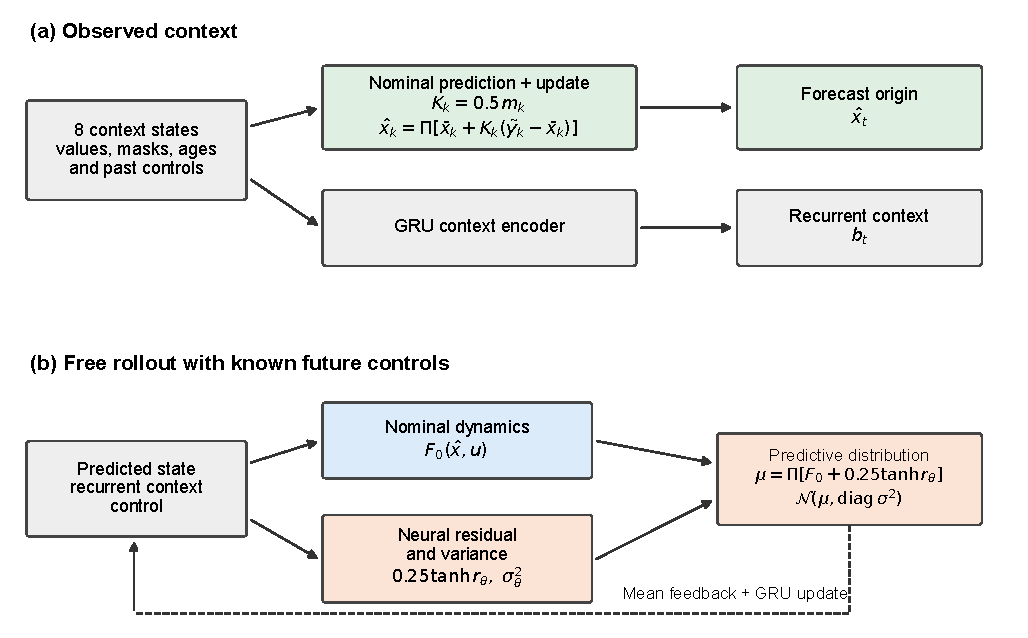
\includegraphics[width=0.96\textwidth]{figures/Fig1.pdf}
\caption{Causal data flow of \method{}. A fixed complementary update is applied only inside the observed context. Missing channels receive zero direct measurement correction before any state-space projection. The filtered forecast origin then initializes a probabilistic nominal-physics plus neural-residual transition, which is rolled out freely for 25 steps using known future controls and no future observations.}
\label{fig:method}
\end{figure*}

\subsection{Forecasting problem}

Let $\vect{x}_t\in\mathbb{R}^{d_x}$ be a physical state and
$\vect{u}_t\in\mathbb{R}^{d_u}$ a recorded control. The observation available
to the model is
\begin{equation}
 \vect{y}_t=\vect{m}_t\odot(\vect{x}_t+\boldsymbol{\epsilon}_t),
\end{equation}
where $\vect{m}_t\in\{0,1\}^{d_x}$ is a channel-wise availability mask and
$\boldsymbol{\epsilon}_t$ is observation noise. Missing entries are filled
causally by the latest available value, producing $\tilde{\vect{y}}_t$; the
mask and elapsed time since observation $\boldsymbol{\delta}_t$ remain explicit
inputs to distinguish imputed values from fresh measurements.

At forecast origin $t$, the model receives eight context states and their past
controls,
\begin{equation}
 \mathcal C_t=\{\tilde{\vect y}_{t-7:t},\vect m_{t-7:t},
 \boldsymbol\delta_{t-7:t},\vect u_{t-7:t-1}\},
\end{equation}
together with known future controls $\vect u_{t:t+H-1}$. It estimates a
diagonal predictive distribution for $\vect{x}_{t+1:t+H}$ under free rollout,
with training horizon $H=25$, using predicted states at subsequent rollout
steps. The flight evaluation additionally extends rollout to $H=50$. All learned
operations use affine statistics estimated from the training split; the
nominal equations are evaluated in physical coordinates and then returned to
normalized coordinates.

\subsection{Mask-gated complementary context filter}

Let $F_0$ denote a nominal dynamics step: fourth-order Runge--Kutta integration
for the controlled benchmark, and the reduced flight model in
Section~\ref{sec:external}. Starting from the first imputed context vector, the
filter alternates nominal prediction and measurement update. For context index
$k>t-7$,
\begin{align}
 \bar{\vect x}_{k} &= F_0(\hat{\vect x}_{k-1},\vect u_{k-1}),\\
 \vect K_k &= \alpha\vect m_k,\qquad \alpha=0.5,\\
 \hat{\vect x}_k &= \Pi\!\left[
 \bar{\vect x}_k+\vect K_k\odot
 (\tilde{\vect y}_k-\bar{\vect x}_k)\right].
 \label{eq:complementary-update}
\end{align}
Thus, before projection, an observed channel receives equal weight from the
nominal prediction and the current measurement, while a missing channel has
exactly zero measurement correction. The projection $\Pi$ is the identity
except for the sine--cosine pendulum representation, which is returned to the
unit circle after each update. This joint projection couples the pendulum
channels and can change a channel whose measurement gain is zero. The zero-gain
statement therefore applies to the direct correction before projection, not
necessarily to the projected state. The gain is
fixed before training, independently of validation and test outcomes.

In parallel, a GRU encodes
$[\tilde{\vect y}_k,\vect m_k,\log(1+\boldsymbol\delta_k),\vect u_{k-1}]$.
Its last hidden state supplies trajectory context to the forecast transition;
the measurement gain remains fixed. The implementation retains the
same unused gain-head parameterization in every controlled-benchmark
fixed-gain sensitivity model,
so comparisons at gains 0, 0.25, 0.5, 0.75, and 1 do not change nominal
capacity. This construction draws on filtering and data-assimilation approaches
\cite{revach2022_kalmannet,cheng2023_machine_learning_with_data_assimilation}
and uses the mask-gated context update to initialize a physics-residual
probabilistic world model.

\subsection{Probabilistic physics-residual rollout}

The last filtered context state initializes a free rollout. At step $h$,
\begin{align}
 \boldsymbol\mu^{p}_{t+h} &= F_0(\hat{\vect x}_{t+h-1},\vect u_{t+h-1}),\\
 [\vect r_{t+h},\vect \ell_{t+h}] &=
 R_\theta([\hat{\vect x}_{t+h-1},\vect u_{t+h-1},\vect b_{t+h-1}]),\\
 \boldsymbol\mu_{t+h} &= \Pi\!\left[
 \boldsymbol\mu^{p}_{t+h}+0.25\tanh(\vect r_{t+h})\right],\\
 \boldsymbol\sigma^2_{t+h} &=
 \max\!\left\{\exp\!\left(\operatorname{clip}(\vect\ell_{t+h},-8,4)\right),
 10^{-6}\right\}.
 \label{eq:residual-rollout}
\end{align}
The fixed coefficient 0.25 bounds every per-step residual to one quarter of a
training standard deviation in normalized coordinates and defines the residual
scale convention used by the architecture. A fixed-weight sensitivity analysis
varies this multiplier at inference to quantify its effect. The predicted mean becomes
the next state, and a GRUCell updates $\vect b$ from that mean and the known
control.

The training loss is the mean diagonal Gaussian negative log likelihood over
all $H$ steps and state channels,
\begin{equation}
\begin{aligned}
 \mathcal L_{\mathrm{NLL}}
 &=\frac{1}{2Hd_x}\sum_{h=1}^{H}\sum_{q=1}^{d_x}
 \left[\log(2\pi\sigma^2_{hq})\right.\\[-0.2em]
 &\qquad\left.+\frac{(x_{hq}-\mu_{hq})^2}{\sigma^2_{hq}}\right].
\end{aligned}
 \label{eq:nll}
\end{equation}
The one-step ablation applies the same loss only at $h=1$ but is still
evaluated by a 25-step free rollout.

When a control objective supplies nonnegative state weights $w_q$, the same
architecture admits the component-weighted loss
\begin{equation}
 \begin{aligned}
 \mathcal L_w={}&\frac{1}{2H\sum_q w_q}
 \sum_{h=1}^{H}\sum_{q=1}^{d_x}w_q \\
 &\times\left[\log(2\pi\sigma^2_{hq})+
 \frac{(x_{hq}-\mu_{hq})^2}{\sigma^2_{hq}}\right].
 \end{aligned}
 \label{eq:weighted-nll}
\end{equation}
The experiments use $w_q=1$ for all channels; Equation~\eqref{eq:weighted-nll}
states how a prespecified downstream cost could change that objective.

\subsection{Causal execution and computational cost}

For each window, execution follows four deterministic stages. First, the GRU
encodes the imputed context together with masks, elapsed times, and past
controls. Second, Equation~\eqref{eq:complementary-update} advances the nominal
state through the same context and applies the mask-gated correction after each
available observation. Third, the final hidden state and filtered state jointly
initialize the residual recurrence. Fourth, Equation~\eqref{eq:residual-rollout}
is iterated for every known future control; predicted means, rather than samples
or targets, feed the next step. Training backpropagates the multi-step NLL
through this entire causal graph. Evaluation uses the identical graph with
gradients disabled, so teacher forcing is absent from both validation and test
rollouts.

Let $T_c$ denote context length, $H$ forecast horizon, $d_b$ recurrent width,
and $C_{F_0}$ the cost of one nominal step. Dense recurrent operations cost
$O((T_c+H)d_b^2)$ per trajectory, while nominal propagation costs
$O((T_c+H)C_{F_0})$. Diagonal mean and variance storage is $O(Hd_x)$; recurrent
working memory at inference is $O(d_b+d_x)$. Thus inference grows linearly in
context and horizon. The fixed filter adds nominal context steps; measured
latency captures their cost in the implementation.

\subsection{Forecast-origin and rollout error}

For an observed scalar channel on which $\Pi$ is the identity, write the
nominal pre-update error as $e_p=\bar x-x$ and measurement error as
$\epsilon=y-x$. Before any non-identity projection, Equation
\eqref{eq:complementary-update} gives the exact post-update error
\begin{equation}
 e_f=(1-\alpha)e_p+\alpha\epsilon.
\end{equation}
Let $v_p=\mathbb E[e_p^2]$, $v_\epsilon=\mathbb E[\epsilon^2]$, and
$c=\mathbb E[e_p\epsilon]$ for zero-mean errors. Then
\begin{equation}
 \mathbb E[e_f^2]=(1-\alpha)^2v_p+\alpha^2v_\epsilon
 +2\alpha(1-\alpha)c.
 \label{eq:filter-mse}
\end{equation}
Provided $v_p+v_\epsilon-2c>0$, the scalar gain minimizing this conditional MSE
over $[0,1]$ is
\begin{equation}
 \alpha^*=\operatorname{clip}_{[0,1]}
 \left(\frac{v_p-c}{v_p+v_\epsilon-2c}\right).
 \label{eq:optimal-gain}
\end{equation}
The fixed value 0.5 is optimal only when $v_p=v_\epsilon$ and $c=0$. In an
adaptive implementation, $v_p$, $v_\epsilon$, and $c$ can be estimated per
channel from training or validation innovations and held fixed for test data,
or predicted causally from sensor metadata. A missing channel has zero gain and
therefore receives no direct measurement-error term. For the pendulum's joint sine--cosine projection,
Equation~\eqref{eq:filter-mse} applies before projection; the projected error
also includes the coupled projection contribution. These dependencies motivate
the fixed-gain sensitivity analysis.

If the rollout transition is locally $L$-Lipschitz and incurs local error
$\eta_h$, the standard recursion yields
\begin{equation}
 \|\hat{\vect x}_{t+H}-\vect x_{t+H}\|
 \le L^H\|\hat{\vect x}_t-\vect x_t\|
 +\sum_{h=0}^{H-1}L^{H-1-h}\eta_h.
\end{equation}
The context filter acts on the initial-error term, while the residual model
must control subsequent local errors. The bound makes these two contributions
to long-horizon forecasting explicit.

For receding-horizon control, Equations~\eqref{eq:complementary-update} and
\eqref{eq:residual-rollout} define an estimator--predictor interface: the
context update supplies the current state, and the residual transition maps a
candidate future control sequence to a state distribution. Prediction error
and channel-level sensitivity quantify the contribution of the fixed-gain
interface in the following experiments.

\subsection{Use of generative AI tools}

Generative AI tools assisted literature screening, manuscript drafting, and
software and analysis-script development. The authors verified the sources,
equations, code, results, and scientific claims, approved the final manuscript,
and take responsibility for its content.

\section{Controlled benchmark design}

\subsection{Controlled systems, corruption, and shift}

We evaluate five action-conditioned nonlinear systems. The damped oscillator
has state $(q,\dot q)$ and dynamics $m\ddot q+c\dot q+kq=u$; the Duffing
oscillator follows $\ddot q+c\dot q+\alpha q+\beta q^3=u$; and the controlled
Van der Pol system follows
$\ddot q=\mu(1-q^2)\dot q-q+g_u u$. The pendulum is represented by
$(\sin\theta,\cos\theta,\dot\theta)$, and the cart--pole by
$(x,\dot x,\theta,\dot\theta)$. Reference trajectories use fourth-order
Runge--Kutta integration with four internal substeps. Initial conditions,
bounded filtered stochastic controls, and physical parameters are generated
from recorded seeds. Shifted parameter intervals are prespecified and disjoint
from training intervals; unit tests verify that separation.

Each seed--system dataset contains 256 training, 64 validation, and 96 ID test
trajectories, plus 96 independently generated OOD test trajectories. A
trajectory has 72 states. Windows contain eight context states and 25 forecast
transitions; training and validation strides are eight and 16, respectively,
whereas evaluation uses one window per trajectory. Split identifiers encode
system, parameter regime, split, trajectory index, and generation seed. No
trajectory crosses splits.

The three evaluation regimes are (i) clean ID context, (ii) ID context with
feature-wise Gaussian noise at 8\% of the mean training-state standard
deviation and a nominal 25\% independent missing-at-random probability, and
(iii) the same corruption with OOD physical parameters. Training context uses
3\% noise and a nominal 10\% missing probability. The first time point of every
generated trajectory is forced observed in every channel so causal last-value
imputation is defined; masks at all subsequent trajectory time points are
sampled independently. A later sliding window can therefore begin at an
unobserved, causally imputed context value. Masks and channel-wise elapsed times
are retained. ID-clean and ID-corrupt evaluations reuse the same underlying 96
trajectories, permitting repeated-measurement resampling. OOD identifiers are
required to be disjoint from ID identifiers.

\subsection{Comparators and sensitivities}

The five broad comparators cover recurrent, normalized, transformer, and
physics-guided transition families. \textbf{RSSM-style} is a compact recurrent
stochastic-style transition. \textbf{SimNorm-style} applies grouped simplex
normalization to its recurrent representation, adapting a representation
principle used by scalable continuous-control world models
\cite{hansen2023_td_mpc2_scalable_robust_world}. \textbf{Transformer-style} uses a
two-layer causal context transformer followed by recurrent free rollout
\cite{micheli2022_transformers_are_sample_efficient_world}. \textbf{PGNN-style}
adds a deterministic neural correction to a nominal physics step
\cite{robinson2022_physics_guided_neural_networks_for}. \textbf{PG-DMM-style} is a
probabilistic physics-residual transition inspired by physics-guided Deep
Markov modeling \cite{liu2022_physics_guided_deep_markov_models}. These are
protocol-matched transition implementations designed for the same explicit-
state forecasting inputs and outputs.

The proposed \textbf{\method} uses gain 0.5. Four fixed-gain sensitivities use
$\alpha\in\{0,0.25,0.75,1\}$, and \textbf{CFR-one-step} changes only the
training horizon. All six CFR variants have hidden width 72 and identical
parameterization; even the inactive fixed-gain head is retained. Comparator
widths are 80 for RSSM-style and SimNorm-style, 48 for Transformer-style, and
84 for PGNN-style and PG-DMM-style.

Architecture, gain, tuning budget, endpoints, and decision thresholds were
fixed using development data before the eight confirmatory seeds were
generated. Development trajectories and model outputs are excluded from the
confirmatory analysis. This separation preserves a direct comparison between
the gain-0.5 model, four fixed-gain sensitivities, and the one-step-trained
variant.

\subsection{Optimization and endpoint definitions}

All models use AdamW, batch size 128, gradient clipping at norm 5, at most 60
epochs, and early stopping after ten epochs without a validation-NLL
improvement of $10^{-5}$. The pre-confirmation tuning archive contains the same
six-trial validation budget for every baseline--system pair. Each baseline uses
its own selected winner. CFR-WM and all CFR sensitivities inherit the selected PGNN-style
winner for the same system. All hyperparameters were fixed before confirmation.

The primary endpoint is NRMSE through horizon 25. Per-feature RMSE is divided
by that feature's standard deviation estimated from the training split only,
then averaged over features. Because stored targets and predictions are already
in those normalized coordinates, the evaluation divisor is one. This avoids
estimating a denominator from the test trajectory and remains defined at
horizon one. Secondary accuracy endpoints are cumulative NRMSE at horizons 1,
5, and 10 and MAE through horizon 25. Probabilistic endpoints are diagonal
Gaussian NLL, empirical 90\% coverage, mean 90\% interval width, and mean
absolute central-interval calibration error over nominal levels 0.1--0.9. A
trajectory is catastrophic when any feature-step absolute error exceeds three
training-set standard deviations.

\subsection{Confirmatory inference}

The confirmation grid contains 11 methods, eight untouched seeds
$(41,53,67,79,83,97,109,113)$, five systems, and three regimes: 440 training
runs, 1,320 aggregate cells, and 126,720 paired trajectory rows. One
deterministic dataset fingerprint is shared by all methods within each
seed--system group, and all 40 such fingerprints must be distinct. The eight
seed-level training/data realizations are the top-level independent clusters;
trajectories are nested observations. Inference conditions on the fixed set of
systems and regimes.

For a seed $s$, let $B_s$ and $C_s$ be the PGNN-style and CFR-WM NRMSE-25 means after
equal weighting of all 15 system--regime cells. The primary estimand is
\begin{equation}
 \Delta_{\mathrm{rel}}=\frac{1}{8}\sum_{s=1}^{8}
 100\frac{B_s-C_s}{B_s}.
 \label{eq:primary-estimand}
\end{equation}
A 5,000-replicate bootstrap resamples seeds globally with replacement. Within
each selected seed and system it resamples paired trajectory identifiers;
ID-clean and ID-corrupt reuse the same sampled identifier vector, while the
disjoint OOD set is resampled independently. Every system--regime cell is
retained, and $B_s$, $C_s$, and their ratio are recomputed in each replicate.
The interval is the two-sided percentile 95\% interval.

H1 states that \method{} improves on the preselected PGNN-style comparator by at least 5\%.
Support requires finite metrics, a lower relative-improvement interval endpoint
of at least 5\%, and a one-sided exact sign-flip $p<0.05$ for the seed effects
after subtracting the 5\% margin. All $2^8$ sign configurations are enumerated
under a prespecified symmetry assumption. Confirmation success is determined
by H1 alone.

H2 is tested only if H1 succeeds. It requires at least 5\% improvement when
pooling ID-corrupt and OOD-corrupt fixed cells, and clean-regime
noninferiority with signed relative-improvement margin $-5\%$. Both components
must meet their respective bootstrap bound and one-sided margin test, with all
metrics finite. The five broad CFR-versus-comparator contrasts form one Holm
family; the five CFR sensitivity/ablation contrasts form another. With eight
clusters, the minimum two-sided exact raw and five-test Holm-adjusted values are
$2/2^8=0.0078125$ and 0.0390625. The 15 system--regime contrasts report paired
effects and unadjusted bootstrap intervals as descriptive estimates.

\subsection{Secondary component and stress analyses}

Six secondary analyses characterize the fitted models. First, two nonlearned
rollouts use the nominal dynamics from either the
final imputed context state or the gain-0.5 filtered context state. Second,
CFR-WM is evaluated with residual multipliers 0, 0.125, 0.25, and 0.5 while
holding the trained weights fixed; the stored 0.25 predictions are reproduced
exactly. Third, a synchronous two-step
all-channel outage is inserted at context indices 3--4, 5--6, or 7--8 of
otherwise clean ID windows and the three start positions are averaged. Fourth,
the pendulum audit measures how often unit-circle projection changes a missing
sine or cosine channel after its zero direct correction. Fifth, stored RTX 5070
batch timings are summarized. Each timing cell places 96 trajectories in one
batch and includes CPU-to-GPU transfer, context encoding, and 25-step rollout,
but excludes data-loader iteration and metric computation. Sixth,
external-flight NLL and marginal interval metrics are recomputed from all 15
final learned checkpoints. These analyses are descriptive and use the original
seed and cell weighting.

\subsection{Reproducibility controls}

The reproducibility contract fixes code hashes, configurations, data identities,
trajectory pairing, and finite-metric checks. Analysis proceeds only after the
complete grid and stored provenance pass these checks.

Execution uses Python 3.11.15 and PyTorch 2.11.0+cu130 on an NVIDIA RTX 5070
Laptop GPU with 8,151 MiB reported memory and an AMD Ryzen 9 9955HX processor.

\section{Controlled benchmark results}

\subsection{Aggregate accuracy}

The analysis includes the complete grid of \ConfirmatoryRuns{}
trained models and \ConfirmatoryTrajectories{} trajectory-level rows. All
prespecified metrics were finite (\AllMetricsFinite), and the 40 seed--system
groups produced \UniqueDataHashes{} distinct data fingerprints while sharing
one fingerprint across methods within each group.

Table~\ref{tab:main-results} reports the seed-balanced mean and standard
deviation for horizons 1, 10, and 25. Across all 11 methods, \BestMethod{}
had the lowest aggregate NRMSE-25 (\BestNRMSE). CFR-WM's mean was
\CFRNRMSE{}, compared with \PGNNNRMSE{} for the preselected PGNN-style comparator.

\begin{table*}[t]
\centering
\caption{Confirmatory accuracy over the fixed five-system, three-regime
benchmark. Entries are means $\pm$ SD across eight seed-level, cell-balanced
aggregates. Bold marks the lowest aggregate NRMSE-25. Parameter counts are means
over the five system-specific input dimensions; all methods received the same six-trial
validation search budget.}
\label{tab:main-results}
\resizebox{\textwidth}{!}{\begin{tabular}{lrrrr}
\toprule
Method & Mean parameters & NRMSE-1 & NRMSE-10 & NRMSE-25 \\
\midrule
CFR-WM & 57694 & 0.039 $\pm$ 0.001 & 0.057 $\pm$ 0.002 & \textbf{0.100 $\pm$ 0.004} \\
CFR-gain-0.25 & 57694 & 0.037 $\pm$ 0.001 & 0.059 $\pm$ 0.002 & 0.103 $\pm$ 0.004 \\
CFR-gain-0.75 & 57694 & 0.047 $\pm$ 0.001 & 0.065 $\pm$ 0.002 & 0.107 $\pm$ 0.005 \\
PGNN-style & 61275 & 0.060 $\pm$ 0.001 & 0.070 $\pm$ 0.002 & 0.110 $\pm$ 0.003 \\
CFR-gain-1 & 57694 & 0.059 $\pm$ 0.001 & 0.073 $\pm$ 0.002 & 0.114 $\pm$ 0.004 \\
PG-DMM-style & 61493 & 0.063 $\pm$ 0.001 & 0.075 $\pm$ 0.002 & 0.114 $\pm$ 0.003 \\
RSSM-style & 62485 & 0.073 $\pm$ 0.002 & 0.090 $\pm$ 0.005 & 0.123 $\pm$ 0.006 \\
Transformer-style & 59708 & 0.074 $\pm$ 0.002 & 0.094 $\pm$ 0.004 & 0.132 $\pm$ 0.009 \\
SimNorm-style & 62485 & 0.074 $\pm$ 0.002 & 0.098 $\pm$ 0.006 & 0.138 $\pm$ 0.013 \\
CFR-gain-0 & 57694 & 0.081 $\pm$ 0.003 & 0.100 $\pm$ 0.003 & 0.144 $\pm$ 0.005 \\
CFR-one-step & 57694 & 0.040 $\pm$ 0.001 & 0.136 $\pm$ 0.050 & 0.278 $\pm$ 0.104 \\
\bottomrule
\end{tabular}}
\end{table*}

For the primary estimand, PGNN-style and CFR-WM
NRMSE-25 are first averaged with equal weight over the 15 prespecified
system--regime cells; their relative improvement is then computed. The
confirmatory point estimate is the arithmetic mean of those eight seed-level
relative improvements rather than the ratio of the two pooled means in
Table~\ref{tab:main-results}.

\subsection{Primary and gated robustness hypotheses}

Against PGNN-style, the seed-mean relative NRMSE-25 improvement was
\PrimaryImprovement\% (95\% paired fixed-cell bootstrap CI
[\PrimaryRelativeCILow\%, \PrimaryRelativeCIHigh\%]). In absolute units,
CFR-WM minus PGNN-style was \PrimaryDifference{} (95\% CI [\PrimaryCILow,
\PrimaryCIHigh]). The exact one-sided sign-flip test against the same 5\%
practical margin gave $p=\PrimaryPValue$. Under the prespecified conjunction of a
5\% interval lower bound, $p<0.05$, and finite metrics, H1 was
\PrimaryDecision.

For the H2 components, the combined corrupt-ID and corrupt-OOD regimes had a
relative effect of \CorruptImprovement\% (95\% CI
[\CorruptRelativeCILow\%, \CorruptRelativeCIHigh\%], one-sided 5\%-margin
$p=\CorruptPValue$). ID-clean had an effect of \CleanImprovement\% (95\% CI
[\CleanRelativeCILow\%, \CleanRelativeCIHigh\%], one-sided signed
$-5\%$-margin $p=\CleanPValue$). Because H2 is hierarchically gated by H1 and
requires both component rules, the robustness hypothesis was
\RobustnessDecision.

Table~\ref{tab:seed-effects} reports the eight independent cluster effects.
Every seed exceeded the 5\% practical threshold.

\begin{table}[t]
\centering
\caption{Seed-level primary effects after equal weighting of the 15
benchmark cells. Positive values favor CFR-WM.}
\label{tab:seed-effects}
\begin{tabular}{rr}
\toprule
Seed & CFR-WM improvement over PGNN-style, \% \\
\midrule
41 & +5.29 \\
53 & +12.76 \\
67 & +12.01 \\
79 & +10.49 \\
83 & +9.69 \\
97 & +6.66 \\
109 & +9.32 \\
113 & +5.56 \\
\bottomrule
\end{tabular}
\end{table}

\begin{figure*}[t]
\centering
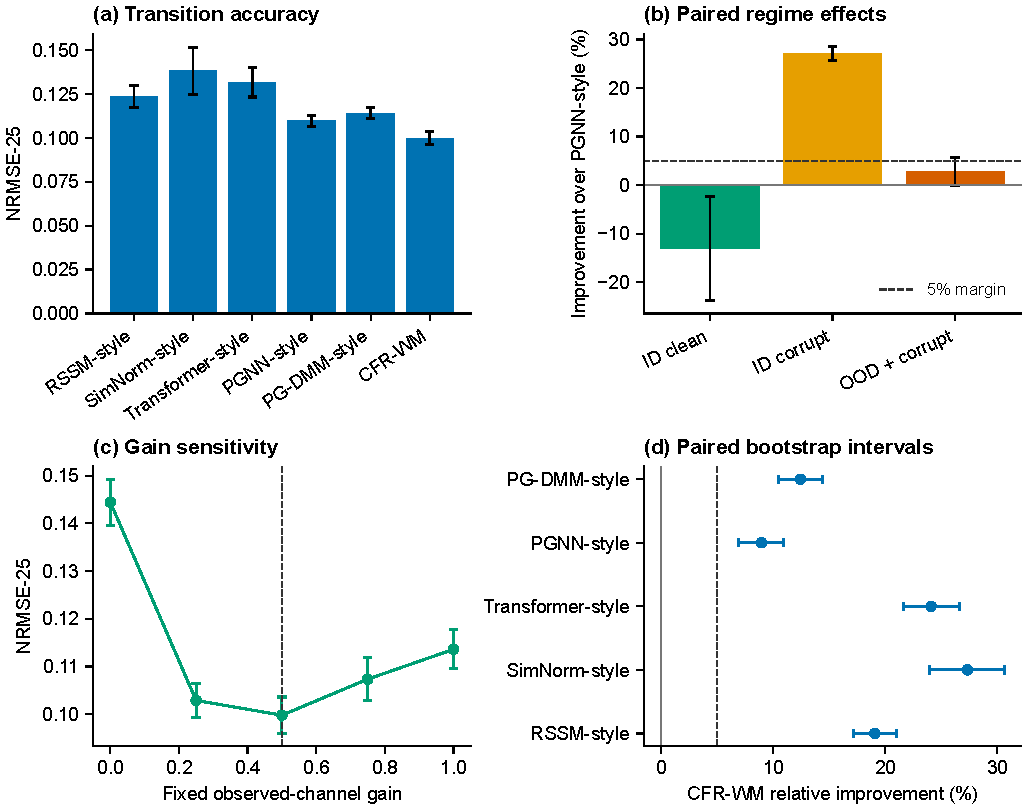
\includegraphics[width=0.96\textwidth]{figures/Fig2.pdf}
\caption{Confirmatory summary. (A) Aggregate transition accuracy for the
six main methods. (B) Paired CFR-WM effects against PGNN-style by regime; positive
values favor CFR-WM. (C) Prespecified fixed-gain sensitivity. (D) Paired
fixed-cell intervals against each broad comparator. Error bars in A--C are
seed-level SD; D uses the nested 95\% bootstrap interval.}
\label{fig:confirmatory-overview}
\end{figure*}

\subsection{Comparator and sensitivity evidence}

Table~\ref{tab:comparator-contrasts} reports every prespecified broad
comparison. Positive relative effects favor CFR-WM. The confidence intervals
retain all fixed cells, whereas the exact two-sided seed sign-flip values are
Holm-adjusted as one five-test family. These secondary comparisons contextualize
the primary PGNN-style contrast.

The PGNN-style row repeats the primary point estimate but uses the
comparator-family bootstrap seed (20260808), whereas H1 uses its prespecified
primary seed (20260805). The estimand and 5,000-replicate resampling scheme are
otherwise identical; the separately sampled interval endpoints differ by at
most 0.01 percentage point after rounding, and only the primary interval enters
the H1 decision.

\begin{table*}[t]
\centering
\caption{CFR-WM relative NRMSE-25 effects against broad comparators. Exact
$p$ values test a zero seed-level difference; Holm adjustment is confined to
this prespecified family of five.}
\label{tab:comparator-contrasts}
\begin{tabular}{lrrr}
\toprule
Reference & Relative effect [95\% CI], \% & Exact $p$ & Holm $p$ \\
\midrule
RSSM-style & +19.08 [+17.16, +20.98] & 0.0078 & 0.0391 \\
SimNorm-style & +27.34 [+24.00, +30.62] & 0.0078 & 0.0391 \\
Transformer-style & +24.09 [+21.65, +26.64] & 0.0078 & 0.0391 \\
PGNN-style & +8.97 [+6.89, +10.96] & 0.0078 & 0.0391 \\
PG-DMM-style & +12.44 [+10.51, +14.39] & 0.0078 & 0.0391 \\
\bottomrule
\end{tabular}
\end{table*}

The lowest aggregate NRMSE-25 among gains $0$, $0.25$, $0.5$, $0.75$, and $1$
occurred at gain \BestGain. Relative to the one-step-trained variant, CFR-WM's
effect was \OneStepImprovement\% (95\% CI [\OneStepRelativeCILow\%,
\OneStepRelativeCIHigh\%], Holm $p=\OneStepHolmP$). Table
\ref{tab:sensitivity-contrasts} gives the complete second five-test family.

\begin{table*}[t]
\centering
\caption{CFR-WM relative NRMSE-25 effects against gain and training-horizon
sensitivities. Positive values favor the proposed gain-0.5 multi-step model.}
\label{tab:sensitivity-contrasts}
\begin{tabular}{lrrr}
\toprule
Reference & Relative effect [95\% CI], \% & Exact $p$ & Holm $p$ \\
\midrule
Gain 0 & +30.89 [+28.95, +32.67] & 0.0078 & 0.0391 \\
Gain 0.25 & +2.97 [+0.88, +5.27] & 0.0312 & 0.0391 \\
Gain 0.75 & +6.97 [+4.77, +9.42] & 0.0078 & 0.0391 \\
Gain 1 & +12.13 [+10.31, +13.92] & 0.0078 & 0.0391 \\
One-step training & +59.38 [+48.88, +68.88] & 0.0078 & 0.0391 \\
\bottomrule
\end{tabular}
\end{table*}

Table~\ref{tab:secondary} reports secondary diagnostics of Gaussian forecast
quality, marginal calibration, and catastrophic-rollout frequency.

\begin{table*}[t]
\centering
\caption{Secondary aggregate diagnostics for the six broad methods. Rates and
scores are seed-balanced over all fixed cells and are not separately tested.}
\label{tab:secondary}
\resizebox{\textwidth}{!}{\begin{tabular}{lrrrr}
\toprule
Method & Parameters & Gaussian NLL & Calibration error & Catastrophic rate \\
\midrule
RSSM-style & 62485 & -0.183 & 0.214 & 0.01\% \\
SimNorm-style & 62485 & -0.246 & 0.206 & 0.01\% \\
Transformer-style & 59708 & -0.279 & 0.202 & 0.01\% \\
PGNN-style & 61275 & -0.385 & 0.248 & 0.00\% \\
PG-DMM-style & 61493 & 0.029 & 0.245 & 0.00\% \\
CFR-WM & 57694 & 0.013 & 0.228 & 0.00\% \\
\bottomrule
\end{tabular}}
\end{table*}

\subsection{Fixed-cell heterogeneity}

Figure~\ref{fig:cell-heterogeneity} retains all 15 system--regime effects. By
the prespecified descriptive guard, CFR-WM was more than 10\% worse than PGNN-style in
\CellsWorseTen{} cells. All three were ID-clean: cart--pole
(\CartpoleCleanChange\% relative change), controlled Van der Pol
(\VanDerPolCleanChange\%), and Duffing (\DuffingCleanChange\%). Conversely,
\IDCorruptFavoredCount{} of \IDCorruptCellCount{} ID-corrupt cells favored
CFR-WM, with descriptive changes from \IDCorruptLeastChange\% to
\IDCorruptMostChange\%. This pattern explains why an aggregate H1 success coexists with
the clean-regime noninferiority result. These cell-level estimates are
descriptive; their unadjusted bootstrap intervals are reported in the appendix
table and machine-readable CSV.

\begin{figure}[t]
\centering
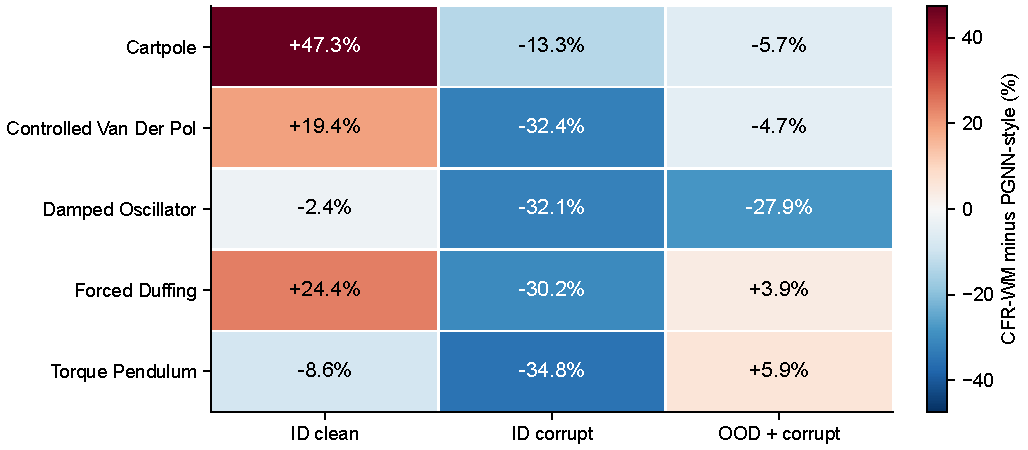
\includegraphics[width=\linewidth]{figures/Fig3.pdf}
\caption{Descriptive CFR-WM change relative to PGNN-style in each fixed benchmark
cell. Negative values mean lower NRMSE-25 for CFR-WM.}
\label{fig:cell-heterogeneity}
\end{figure}

\subsection{Component analyses and stress tests}

Table~\ref{tab:posthoc-baseline} separates the context filter from the learned
residual. The gain-0.5 filter followed by nominal rollout reaches 0.111
NRMSE-25, below both CFR-WM (0.119) and PGNN-style (0.132). Evaluating the
trained CFR-WM weights at their stored residual multiplier of 0.25 reproduces the stored
cell means with maximum absolute difference
\ResidualReconstructionDifference{}. Across the four tested inference
multipliers, the lowest aggregate and regime-specific means occur at scale
\PosthocBestResidualScale{}. The learned residual therefore increases the
fixed-weight mean error in this analysis.

\begin{table*}[t]
\centering
\caption{Classical baselines and inference-time residual-scale
analysis. Entries are seed-balanced mean NRMSE-25 across the indicated fixed
cells. The scale analysis holds trained CFR-WM weights fixed and isolates the
residual contribution.}
\label{tab:posthoc-baseline}
\resizebox{\textwidth}{!}{\begin{tabular}{lrrrr}
\toprule
Analysis and variant & All & Clean & ID corrupt & OOD corrupt \\
\midrule
Nominal, final imputation & 0.137 & 0.040 & 0.151 & 0.221 \\
Complementary filter + nominal & 0.111 & 0.042 & 0.092 & 0.201 \\
PGNN-style & 0.132 & 0.052 & 0.134 & 0.211 \\
CFR-WM & 0.119 & 0.055 & 0.097 & 0.204 \\
\midrule
CFR-WM, inference scale 0 & 0.111 & 0.042 & 0.092 & 0.201 \\
CFR-WM, inference scale 0.125 & 0.113 & 0.046 & 0.093 & 0.202 \\
CFR-WM, inference scale 0.25 & 0.119 & 0.055 & 0.097 & 0.204 \\
CFR-WM, inference scale 0.5 & 0.135 & 0.079 & 0.113 & 0.213 \\
\bottomrule
\end{tabular}}
\end{table*}

The synchronous two-step all-channel outage produces a 2.7\% increase over
clean-context CFR-WM, compared with 51.9\% for PGNN-style
(Table~\ref{tab:structured-outage}). For the pendulum, unit-circle projection
changes \ProjectionChangedFraction\% of the \ProjectionMissingEntries{}
missing sine/cosine entries after the direct correction. The mean, 95th
percentile, and maximum absolute normalized changes are \ProjectionMeanChange{},
\ProjectionPChange{}, and \ProjectionMaxChange{}, respectively. Thus the mask
sets the direct measurement gain to zero, but projection can still alter a
missing coordinate.

\begin{table*}[t]
\centering
\caption{Clean-ID performance after a synchronous two-step all-channel context
outage. Means $\pm$ SD and relative changes are across eight seed-level
aggregates after averaging systems and the three outage positions.}
\label{tab:structured-outage}
\begin{tabular}{lrr}
\toprule
Method & Outage NRMSE-25 & Change from clean (\%) \\
\midrule
PGNN-style & 0.079 $\pm$ 0.004 & +51.9 \\
CFR-WM & 0.057 $\pm$ 0.003 & +2.7 \\
\bottomrule
\end{tabular}
\end{table*}

Table~\ref{tab:latency} reports the stored measured runtime. CFR-WM requires
\CFRLatencyMean{} $\pm$ \CFRLatencySD{} ms per trajectory, including its
nominal context filtering. The measurement is a throughput statistic for one
96-trajectory GPU batch, not single-trajectory online latency.

\begin{table}[t]
\centering
\caption{Measured 25-step rollout time on the RTX 5070. Each cell uses one
batch of 96 trajectories and includes transfer, context encoding, and rollout;
SD is across seed-level cell-balanced means.}
\label{tab:latency}
\begin{tabular}{lrr}
\toprule
Method & ms/trajectory & SD \\
\midrule
RSSM-style & 0.110 & 0.006 \\
SimNorm-WM & 0.113 & 0.005 \\
Transformer-style & 0.109 & 0.007 \\
PGNN-style & 0.347 & 0.037 \\
PG-DMM-style & 0.344 & 0.036 \\
CFR-WM & 0.416 & 0.015 \\
\bottomrule
\end{tabular}
\end{table}

\section{External evaluation on measured drone flights}
\label{sec:external}

\subsection{Data, held-out trajectories, and physical prior}

We extend the controlled study to the NanoDrone benchmark, which records
Crazyflie 2.1 Brushless flights using motion capture and onboard sensors
\cite{busetto2026_nanodrone}. The released records include the dataset authors'
offline synchronization, 100\,Hz resampling, motor--acceleration alignment,
and zero-phase low-pass filtering. We retain these records and predict their
recorded state estimates. Position, velocity, rotation-vector orientation,
and body angular velocity form a 12-coordinate state; four motor angular
speeds are the inputs.

Complete flights define the split. Runs 1--3 of Square, Random, and Chirp
provide nine training records (41,700 samples); run 4 of each supplies three
validation records (13,899 samples). Three Melon flights (19,497 samples)
test a trajectory family absent from training. This validation holdout is an
addition to the authors' training/test partition. Windows remain within
flights, and normalization uses training samples only.

The nominal model combines gravity with thrust along the body vertical axis:
\begin{equation}
 a_t=c_T R(r_t)e_3\sum_{j=1}^{4}\omega_{j,t}^{2}-g e_3.
 \label{eq:flight-prior}
\end{equation}
The kinematic updates are
$v_{t+1}=v_t+\Delta t\,a_t$ and
$p_{t+1}=p_t+\Delta t\,v_t+\tfrac12\Delta t^2a_t$.
Here $r_t$ is the rotation vector, $\omega_{j,t}$ is motor speed,
$g=9.81\,\mathrm{m\,s^{-2}}$, and $\Delta t=0.01$\,s. A nonnegative
least-squares fit on training transitions gives
$c_T=8.31887655\times10^{-7}$ in
$(\mathrm{m\,s^{-2}})/(\mathrm{rad\,s^{-1}})^2$.
Orientation advances by quaternion composition under constant body angular
velocity. The prior omits angular acceleration, drag, and motor lag, adding
structural mismatch to the parameter mismatch studied in the simulations.

\subsection{Matched comparisons and evaluation protocol}

The flight implementation uses a width-64 recurrent encoder and residual
transition. Three learned models share \ExternalLearnedParameters{} parameters:
CFR-WM with gain 0.5, an unfiltered physics-residual model, and a data-only
recurrent transition. The latter replaces the nominal physics step with a
learned increment; the unfiltered model starts from the final imputed
measurement. All three use the same encoder, bounded correction, and
diagonal-Gaussian likelihood. The context GRU receives 40 features; a
width-64 GRU cell advances the hidden state from 12 predicted coordinates and
four inputs. An $80\!\to\!64\!\to\!64\!\to\!24$ SiLU head outputs
12 corrections and 12 log variances. Corrections use $0.25\tanh(\cdot)$ in
normalized coordinates, and log variances are clipped to $[-8,4]$.
A nominal-only forecast supplies a fourth
reference. These matched implementations follow the physics, hybrid, and
recurrent families represented in the NanoDrone benchmark.

Each window contains eight context states. Last-value imputation and elapsed
missingness times are computed within each flight before window extraction,
so an imputed entry can retain an observation preceding the eight-state
context. Training uses an equal mixture of recorded contexts and contexts
with Gaussian noise of 0.05 training standard deviations per coordinate and
10\% independent missingness. Controls and targets are unchanged. All learned
models train on 25-step rollouts with stride 10, AdamW, batch size 256, at most
40 epochs, and eight-epoch early stopping. Each method selects between
learning rates 0.001 and 0.003 by validation NLL using development seed 17,
then trains with five final seeds (131, 149, 167, 181, 199).

Evaluation uses four paired context conditions: as recorded, Gaussian noise
only (0.1 training standard deviations), missingness only (30\%), and their
combination. The same perturbation realization is shared across methods and
training seeds. Known recorded motor inputs drive free forecasts through
25 and 50 steps (0.25 and 0.5\,s), with test stride 50. For flight $f$, model
$m$, and horizon $H$, the external score is
\begin{equation}
\begin{aligned}
 E_{m,f,H}=\left[\frac{1}{12H N_f}
 \sum_{i=1}^{N_f}\sum_{h=1}^{H}\sum_{d=1}^{12}\right.\\[-0.2em]
 \left.\left(\frac{\widehat{x}_{m,i,h,d}-x_{i,h,d}}{s_d}\right)^2
 \right]^{1/2},
\end{aligned}
 \label{eq:external-score}
\end{equation}
where $s_d$ is the training standard deviation. This score takes one root
after pooling normalized squared errors; the controlled study instead
averages feature-wise normalized RMSE. External summaries first give the
three flights equal weight, then report the mean and sample SD across five
training seeds. Position and velocity scores use root-mean-square Euclidean
error in physical units. Paired relative improvements are averaged across
seeds after the same flight weighting.

The external comparisons use no controlled-benchmark test data for training or
model selection and are reported descriptively.

\subsection{Flight forecasting results}

Table~\ref{tab:external-results} reports all eight condition--horizon
comparisons. Each learned model has lower mean full-state NRMSE than the
nominal forecast. The unfiltered residual model has lower mean full-state
NRMSE than CFR-WM in all eight comparisons. With recorded contexts at 50 steps,
their scores are \ExternalUnfilteredRecordedLongNRMSEMean{} and
\ExternalCFRRecordedLongNRMSEMean{}, respectively. Combined noise and
missingness narrows this difference to
\ExternalUnfilteredCombinedLongNRMSEMean{} versus
\ExternalCFRCombinedLongNRMSEMean{}.
CFR-WM improves over the data-only recurrent model at 25 steps under added
noise and combined corruption, but its mean error is higher at 50 steps
in all four conditions.

The physical-unit scores distinguish position and velocity behavior
(Table~\ref{tab:external-physical}; Figure~\ref{fig:external-flight}).
CFR-WM has the lowest 50-step position error among the three learned models
in all four conditions. Under combined corruption, its position error is
\ExternalCFRCombinedLongPositionMean{}\,m, compared with
\ExternalUnfilteredCombinedLongPositionMean{}\,m for the unfiltered model.
The nominal prior has lower position error than the learned models on
recorded and missing-only contexts, despite its higher full-state error.
Velocity errors show a different ordering: CFR-WM is worse than the
unfiltered model on recorded and missing-only contexts, and nearly tied
under noise and combined corruption. Thus, the position benefit coexists
with a full-state accuracy cost on these held-out flights.

The 50-step probabilistic diagnostics quantify forecast calibration
(Table~\ref{tab:external-uncertainty}). CFR-WM has higher Gaussian
NLL, lower nominal 90\% coverage, narrower intervals, and higher calibration
error than the unfiltered residual model in every context condition. Its
coverage ranges from 0.524 to 0.667, well below 0.9. The diagonal likelihood
therefore produces undercovered marginal intervals on these held-out flights;
lower position error does not imply reliable joint-state uncertainty.

\begin{table*}[t]
\centering
\caption{External flight NRMSE (Equation~\ref{eq:external-score}). Entries
are means $\pm$ SD across five training seeds after equal weighting of three
held-out flights. The nominal forecast is deterministic. All four context
conditions and both horizons are retained.}
\label{tab:external-results}
\resizebox{\textwidth}{!}{\begin{tabular}{llrrrr}
\toprule
Context & Horizon & CFR-WM & Unfiltered & Recurrent & Nominal \\
\midrule
As recorded & 25 & $0.389 \pm 0.012$ & $0.376 \pm 0.010$ & $0.388 \pm 0.008$ & $0.488$ \\
As recorded & 50 & $0.530 \pm 0.016$ & $0.518 \pm 0.019$ & $0.519 \pm 0.006$ & $0.790$ \\
Noise & 25 & $0.393 \pm 0.012$ & $0.387 \pm 0.010$ & $0.398 \pm 0.008$ & $0.498$ \\
Noise & 50 & $0.532 \pm 0.017$ & $0.523 \pm 0.018$ & $0.527 \pm 0.006$ & $0.797$ \\
Missing & 25 & $0.397 \pm 0.011$ & $0.386 \pm 0.008$ & $0.395 \pm 0.005$ & $0.495$ \\
Missing & 50 & $0.537 \pm 0.014$ & $0.527 \pm 0.020$ & $0.526 \pm 0.007$ & $0.792$ \\
Noise + missing & 25 & $0.401 \pm 0.011$ & $0.397 \pm 0.008$ & $0.405 \pm 0.005$ & $0.506$ \\
Noise + missing & 50 & $0.540 \pm 0.014$ & $0.534 \pm 0.019$ & $0.533 \pm 0.006$ & $0.799$ \\
\bottomrule
\end{tabular}}
\end{table*}

\begin{table*}[t]
\centering
\caption{External 50-step position and velocity error in physical units,
using the same flight and seed weighting as Table~\ref{tab:external-results}.}
\label{tab:external-physical}
\resizebox{\textwidth}{!}{\begin{tabular}{lrrrr}
\toprule
& \multicolumn{2}{c}{Position RMSE (m)} & \multicolumn{2}{c}{Velocity RMSE (m/s)} \\
Context & CFR-WM & Unfiltered & CFR-WM & Unfiltered \\
\midrule
As recorded & $0.078 \pm 0.003$ & $0.083 \pm 0.010$ & $0.249 \pm 0.015$ & $0.233 \pm 0.009$ \\
Noise & $0.091 \pm 0.003$ & $0.115 \pm 0.007$ & $0.257 \pm 0.014$ & $0.258 \pm 0.007$ \\
Missing & $0.081 \pm 0.005$ & $0.095 \pm 0.022$ & $0.259 \pm 0.014$ & $0.243 \pm 0.009$ \\
Noise + missing & $0.094 \pm 0.004$ & $0.125 \pm 0.017$ & $0.267 \pm 0.014$ & $0.268 \pm 0.009$ \\
\bottomrule
\end{tabular}}
\end{table*}

\begin{table*}[t]
\centering
\caption{External 50-step probabilistic diagnostics. Coverage and width refer
to marginal nominal 90\% Gaussian intervals; calibration error averages
absolute central-interval coverage error over nominal levels 0.1--0.9. Entries
are means across five seeds after equal weighting of the three held-out flights.}
\label{tab:external-uncertainty}
\resizebox{\textwidth}{!}{\begin{tabular}{llrrrr}
\toprule
Condition & Method & NLL & Cov. & Width & Cal. error \\
\midrule
Recorded & CFR-WM & 2.264 & 0.608 & 0.453 & 0.178 \\
Recorded & Unfiltered residual & 0.794 & 0.716 & 0.526 & 0.099 \\
Noise & CFR-WM & 2.994 & 0.524 & 0.454 & 0.242 \\
Noise & Unfiltered residual & 2.361 & 0.565 & 0.528 & 0.217 \\
Missing & CFR-WM & 1.829 & 0.667 & 0.534 & 0.123 \\
Missing & Unfiltered residual & 0.735 & 0.779 & 0.685 & 0.053 \\
Combined & CFR-WM & 2.200 & 0.613 & 0.535 & 0.184 \\
Combined & Unfiltered residual & 1.130 & 0.703 & 0.688 & 0.124 \\
\bottomrule
\end{tabular}}
\end{table*}

\begin{figure*}[t]
\centering
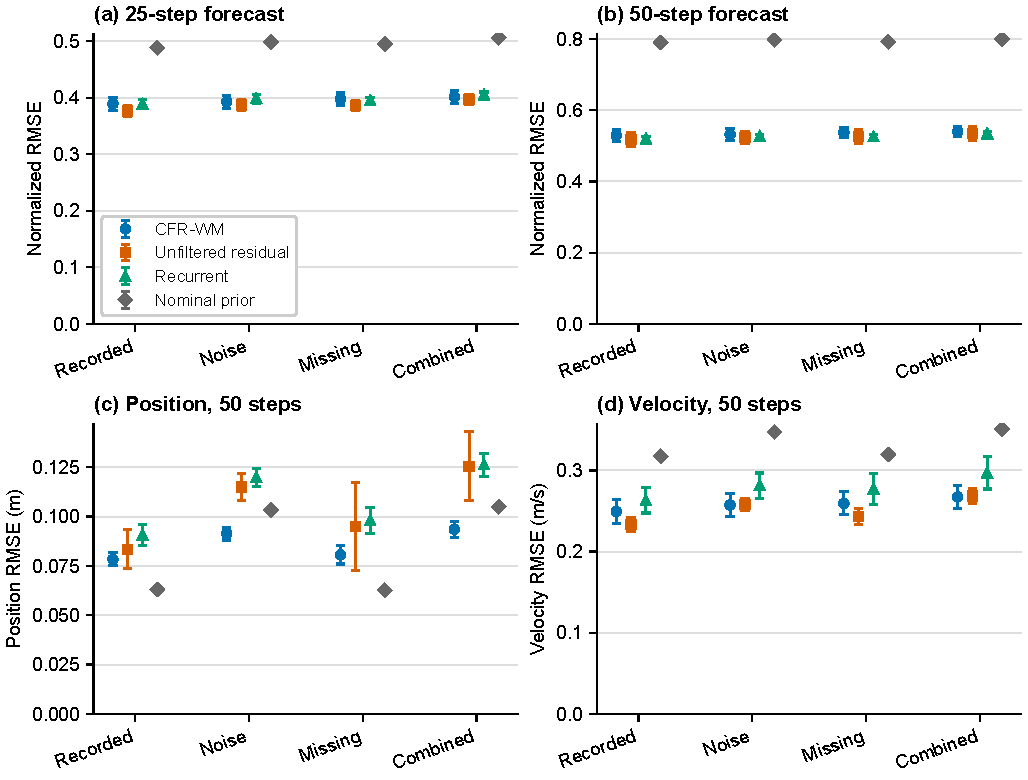
\includegraphics[width=\textwidth]{figures/Fig4.pdf}
\caption{Prediction on the held-out Melon flights: both normalized-error
horizons and 50-step position and velocity errors. Error bars describe
training-seed variation on the same three test flights.}
\label{fig:external-flight}
\end{figure*}

\section{Discussion}

The confirmatory analysis \PrimaryInterpretation. Against the preselected
PGNN-style comparator, the lower bootstrap endpoint clears the 5\% practical
margin and the exact seed-level test rejects that margin. The classical
baseline refines the interpretation of this result. A gain-0.5
context filter followed by the nominal transition reaches 0.111 NRMSE-25,
compared with 0.119 for CFR-WM and 0.132 for PGNN-style. The confirmatory H1
remains supported for its prespecified comparison. The component analysis
attributes the aggregate advantage to forecast-origin filtering rather than to
the learned residual transition.

The fixed-weight scale analysis strengthens that attribution. Removing the
residual at inference gives the lowest mean in clean ID, corrupt ID, corrupt
OOD, and the aggregate; increasing the multiplier from 0 to 0.5 monotonically
increases aggregate NRMSE-25. With transition weights held fixed, the fitted
correction increases the reported cell-balanced point error. The nominal prior
and context correction capture the useful structure in this benchmark.

The regime decomposition explains when the filter helps relative to PGNN-style.
The corrupted and shifted regimes improve by \CorruptImprovement\%, whereas
the clean regime changes by \CleanImprovement\%; consequently H2
\RobustnessInterpretation. The synchronous two-step outage produces only a
2.7\% increase over clean-context CFR-WM, versus 51.9\% for PGNN-style. This
extends the missing-at-random evidence to a short, synchronized loss of all
channels and indicates that nominal context propagation is valuable during
brief sensor interruptions.

Equation~\eqref{eq:optimal-gain} turns the gain trade-off into an estimator
design rule. Equal trust is optimal only for equal prediction and measurement
error variances with zero cross-covariance. Per-channel estimates of
$v_p$, $v_\epsilon$, and $c$ from training or validation innovations would
produce fixed channel gains without using test outcomes; a causal network could
instead condition them on current sensor metadata. Either construction matches
the observed heterogeneity better than one scalar gain. The pendulum audit also
shows why gain semantics and state constraints must be separated: 75.4\% of
missing sine/cosine entries change under the subsequent unit-circle projection,
even though their direct measurement correction is exactly zero.

The measured-flight evaluation exposes a state-component and uncertainty
trade-off. The matched unfiltered residual model has lower mean full-state
NRMSE in every condition--horizon comparison, whereas CFR-WM has lower 50-step
position error in all four conditions. On recorded contexts, velocity error
rises from \ExternalUnfilteredRecordedLongVelocityMean{} to
\ExternalCFRRecordedLongVelocityMean{}\,m\,s$^{-1}$. At the same horizon,
CFR-WM's nominal 90\% marginal coverage is only 0.524--0.667 and is below the
unfiltered model in all four conditions. Narrower intervals accompany higher
NLL and calibration error, consistent with missing cross-state dependence and
unrepresented model-form error in the diagonal Gaussian forecast.

These results connect estimator design to the control objective. Uniform NLL
weights every normalized state component equally, while a controller can value
position, velocity, or constraint-related coordinates differently.
Equation~\eqref{eq:weighted-nll} makes such weights explicit and requires them
to be fixed from the downstream specification rather than selected from test
performance. Correlated covariance or calibrated prediction sets would also be
needed when constraints depend jointly on several state coordinates.

The measured runtime places CFR-WM at
\CFRLatencyMean{}\,ms per trajectory for an eight-step context and 25-step
rollout on the stated GPU and represents throughput for 96 simultaneous
trajectories. Online control requires separate timing and closed-loop tests for
a specified controller, plant, sampling deadline, and disturbance model
\cite{hewing2020_learning_mpc}.

\section{Limitations}

The controlled evidence concerns five equation families with known inputs and
eight independent data-training seed clusters. The secondary component analyses
use the same trained checkpoints and are descriptive. The structured
missingness test is a synchronous two-step
outage inside an eight-step context. Longer bursts, informative dropout, sensor-
specific failure, and delayed measurements are not represented.

The measured-flight evidence contains three held-out trajectories from one
platform and collection session. Targets are the dataset authors'
offline-preprocessed state estimates, and forecasts use recorded future motor
inputs. The resulting scope is offline prediction on one platform and
collection session; raw-sensor estimation, cross-platform transfer, and
closed-loop control require separate evaluation.

The flight prior omits angular acceleration, drag, and motor lag. A uniform
fixed gain cannot track channel- or time-dependent reliability. The
diagonal-Gaussian output omits cross-state covariance and multimodality, and its
50-step marginal intervals under-cover on the held-out flights. Unit-circle
projection couples pendulum coordinates after the mask-gated correction. No
stability certificate follows from the bounded residual or the reported
open-loop prediction errors.

\section{Conclusion}

CFR-WM combines a gain-0.5 context filter with nominal-physics and learned-
residual rollout. Against the prespecified PGNN-style comparator, it improves
cell-balanced NRMSE-25 by \PrimaryImprovement\% (95\% CI
[\PrimaryRelativeCILow\%, \PrimaryRelativeCIHigh\%]), so H1 is supported. H2
is not supported because clean-condition noninferiority fails.

The classical baseline identifies the source of the benchmark result.
The gain-0.5 filter followed by nominal rollout records 0.111 NRMSE-25, below
CFR-WM's 0.119, and residual scale zero is best in every reported regime.
The benchmark gain therefore arises from forecast-origin filtering; the tested
residual adds no point-accuracy benefit.
A short synchronous all-channel outage increases CFR-WM error by 2.7\%, versus
51.9\% for PGNN-style.

On held-out flights, CFR-WM lowers 50-step position error in all four context
conditions but raises full-state NRMSE in all eight condition--horizon
comparisons and yields undercovered 50-step intervals. Together, these findings
motivate channel-specific gains derived from prediction--measurement error
statistics, state weights tied to the control objective, and covariance models
that represent cross-state uncertainty.

\backmatter
\begin{appendices}
% Keep Hyperref destinations unique when the Springer class resets appendix counters.
\renewcommand{\theHtable}{appendix.\arabic{table}}
\renewcommand{\theHfigure}{appendix.\arabic{figure}}
\renewcommand{\theHequation}{appendix.\arabic{equation}}
\section{Benchmark specification}

Table~\ref{tab:systems} records the simulator time step and nominal
parameterization; Table~\ref{tab:parameter-ranges} gives every sampled training
and OOD interval. All OOD intervals are non-overlapping on every named shifted
parameter. These ranges define the fixed benchmark.

\begin{table*}[ht]
\centering
\caption{Controlled-system definitions. $u$ is scalar in every system.}
\label{tab:systems}
\resizebox{\textwidth}{!}{%
\begin{tabular}{llll}
\toprule
System & State & $\Delta t$ & Nominal parameters \\
\midrule
Damped oscillator & $(q,\dot q)$ & 0.050 & $m=1.0,\; k=1.6,\; c=0.18$ \\
Forced Duffing & $(q,\dot q)$ & 0.040 & $\alpha=-1.0,\;\beta=1.0,\;c=0.25$ \\
Controlled Van der Pol & $(q,\dot q)$ & 0.035 & $\mu=1.2,\;g_u=1.0$ \\
Torque pendulum & $(\sin\theta,\cos\theta,\dot\theta)$ & 0.040 & $g=9.81,\;l=1.0,\;m=1.0,\;c=0.12$ \\
Cart--pole & $(x,\dot x,\theta,\dot\theta)$ & 0.025 & $g=9.81,\;m_c=1.0,\;m_p=0.1,\;l/2=0.5,\;c=0.04$ \\
\bottomrule
\end{tabular}}
\end{table*}

\begin{table*}[ht]
\centering
\scriptsize
\caption{Complete independently sampled physical-parameter intervals. Symbols
follow Table~\ref{tab:systems}; $g_u$ is the Van der Pol control gain.}
\label{tab:parameter-ranges}
\resizebox{\textwidth}{!}{%
\begin{tabular}{lll}
\toprule
System & Training interval & OOD interval \\
\midrule
Damped oscillator & $m\in[0.90,1.10],\ k\in[1.40,1.80],\ c\in[0.14,0.22]$ & $m\in[1.25,1.45],\ k\in[2.05,2.35],\ c\in[0.26,0.34]$ \\
Forced Duffing & $\alpha\in[-1.10,-0.90],\ \beta\in[0.90,1.10],\ c\in[0.20,0.30]$ & $\alpha\in[-0.75,-0.60],\ \beta\in[1.25,1.45],\ c\in[0.34,0.44]$ \\
Controlled Van der Pol & $\mu\in[1.00,1.40],\ g_u\in[0.90,1.10]$ & $\mu\in[1.65,1.95],\ g_u\in[1.25,1.45]$ \\
Torque pendulum & $g\in[9.65,9.95],\ l\in[0.90,1.10],\ m\in[0.90,1.10],\ c\in[0.08,0.16]$ & $g\in[10.25,10.55],\ l\in[1.25,1.45],\ m\in[1.25,1.45],\ c\in[0.20,0.28]$ \\
Cart--pole & $g\in[9.65,9.95],\ m_c\in[0.90,1.10],\ m_p\in[0.085,0.115],\ l/2\in[0.45,0.55],\ c\in[0.02,0.06]$ & $g\in[10.25,10.55],\ m_c\in[1.25,1.45],\ m_p\in[0.135,0.160],\ l/2\in[0.65,0.78],\ c\in[0.075,0.105]$ \\
\bottomrule
\end{tabular}}
\end{table*}

The action generator is a bounded first-order filtered process. At step $t$, a Gaussian innovation with scale $0.55$ times the system action limit is combined with the previous action using coefficients 0.18 and 0.82, then clipped. Limits are 1.5, 1.8, 1.2, 2.2, and 8.0 for the systems in Table~\ref{tab:systems}. This produces persistent excitation independently of the simulated state and defines the control-input distribution.

Train/validation/test separation occurs before window construction. A root NumPy \texttt{SeedSequence} spawns distinct split generators, which in turn spawn one generator per trajectory. The OOD test has a separate root seed. Observation corruption uses another recorded seed after state generation. Consequently, changing an observation-noise level does not change the underlying clean ID trajectory, and all methods see exactly the same corruption draw within a condition.

\section{Confirmatory grid}

The prespecified grid comprises 11 methods, eight seeds (41, 53, 67, 79, 83, 97, 109, and 113), five systems, and three test regimes. It therefore contains 440 fitted models, 1,320 aggregate evaluation cells, and 126,720 trajectory-level rows. Each seed--system dataset contains 256 training, 64 validation, and 96 test trajectories of 72 time steps. Models receive eight context steps and predict 25 steps open loop. Training observations use noise equal to 3\% of the fixed training-state scale and a nominal 10\% independent missing probability; the corrupt regimes use 8\% observation noise and a nominal 25\% probability. The first time point of each generated trajectory is forced observed in every channel, with independent masks sampled at all subsequent trajectory times; a later sliding-window context can begin with an imputed value. ID-clean and ID-corrupt evaluations share trajectory identifiers; the OOD trajectory set is disjoint.

The five broad comparators are compact, protocol-matched RSSM-style,
SimNorm-style, Transformer-style, PGNN-style, and PG-DMM-style transitions. Five
prespecified CFR sensitivities test gains $0$, $0.25$, $0.75$, and $1$, plus a
one-step-trained gain-0.5 model. CFR-WM retains the unused learned-gain-head
parameters to maintain identical parameter counts across fixed-gain comparisons.

All methods ingest normalized context values, masks, log-one-plus elapsed times,
and actions. Except for the Transformer-style encoder, context is encoded by a
GRU; open-loop recurrent updates use a GRUCell. Every MLP has two hidden linear
layers with SiLU activation. Table~\ref{tab:architectures} lists the remaining
architecture-specific choices.

\begin{table*}[ht]
\centering
\scriptsize
\caption{Exact compact transition architectures used in the confirmatory grid.
The bounded correction is $0.25\tanh(\cdot)$ and all forecast covariances are
diagonal.}
\label{tab:architectures}
\resizebox{\textwidth}{!}{%
\begin{tabular}{llll}
\toprule
Method & Width & Context representation & Forecast transition and variance \\
\midrule
RSSM-style & 80 & GRU; sigmoid feature scaling & data-only MLP mean/log-variance; GRUCell rollout \\
SimNorm-style & 80 & GRU; eight-group simplex projection & data-only MLP mean/log-variance; GRUCell rollout \\
Transformer-style & 48 & two causal layers, four heads, FF width 96, GELU, dropout 0 & data-only MLP mean/log-variance; GRUCell rollout \\
PGNN-style & 84 & GRU & nominal one-substep RK4 plus deterministic residual MLP; learned constant log-variance \\
PG-DMM-style & 84 & GRU & nominal one-substep RK4 plus residual mean/log-variance MLP \\
CFR-WM and gain sensitivities & 72 & GRU states plus mask-gated fixed-gain context update & nominal one-substep RK4 plus residual mean/log-variance MLP \\
\bottomrule
\end{tabular}}
\end{table*}

For CFR-WM, observed context channels use gain 0.5 and missing channels use
gain 0 exactly. The learned gain head remains instantiated but is inactive.
The four gain sensitivities change only the observed-channel gain; the
one-step sensitivity changes only the likelihood horizon.

\section{Hyperparameter search}

The same six learning-rate/weight-decay trials were run on development seed 11
for every system--baseline pair (Table~\ref{tab:tuning-grid}). The stored
reliability-loss weight is shown because it is part of the generic training
configuration, but it is inactive for all confirmatory methods in this paper.
Each baseline uses the validation-NLL winner in
Table~\ref{tab:tuning-winners}; CFR-WM and all CFR sensitivities inherit the
PGNN-style winner for the same system.

\begin{table}[ht]
\centering
\caption{Six-trial optimization grid.}
\label{tab:tuning-grid}
\begin{tabular}{rrrr}
\toprule
Trial & Learning rate & Weight decay & Stored $\lambda_{\mathrm{rel}}$ \\
\midrule
0 & $3\times10^{-4}$ & $10^{-6}$ & 0.1 \\
1 & $6\times10^{-4}$ & $10^{-5}$ & 0.2 \\
2 & $10^{-3}$ & $10^{-5}$ & 0.2 \\
3 & $1.5\times10^{-3}$ & $10^{-4}$ & 0.3 \\
4 & $2\times10^{-3}$ & $10^{-5}$ & 0.4 \\
5 & $3\times10^{-3}$ & $10^{-4}$ & 0.2 \\
\bottomrule
\end{tabular}
\end{table}

\begin{table*}[ht]
\centering
\caption{Selected trial index by system and protocol-matched baseline.}
\label{tab:tuning-winners}
\resizebox{\textwidth}{!}{%
\begin{tabular}{lrrrrr}
\toprule
System & RSSM-style & SimNorm-style & Transformer-style & PGNN-style & PG-DMM-style \\
\midrule
Damped oscillator & 3 & 2 & 4 & 5 & 1 \\
Forced Duffing & 5 & 4 & 5 & 5 & 5 \\
Controlled Van der Pol & 5 & 5 & 5 & 5 & 0 \\
Torque pendulum & 5 & 5 & 5 & 5 & 4 \\
Cart--pole & 5 & 5 & 5 & 5 & 5 \\
\bottomrule
\end{tabular}
}
\end{table*}

\section{Confirmatory estimands and decisions}

H1 is the sole confirmation gate. It asks whether CFR-WM improves fixed-training-scale NRMSE-25 over the preselected PGNN-style comparator by at least 5\%. Within each seed, PGNN-style and CFR-WM are averaged with equal weight over all 15 fixed system--regime cells; the primary point estimate is the arithmetic mean of the eight seed-specific relative improvements. H1 requires finite metrics, a 95\% bootstrap lower endpoint of at least 5\%, and a one-sided exact sign-flip $p<0.05$ for the 5\% margin.

H2 is a hierarchically gated robustness claim. Conditional on H1, the combined corrupt and parameter-shifted regimes must satisfy the same 5\% improvement rule, while ID-clean performance must be noninferior under a signed relative margin of $-5\%$. Both components require their corresponding bootstrap lower endpoint to meet or exceed the margin and a one-sided exact sign-flip $p<0.05$. If H1 fails, H2 is not supported irrespective of its component estimates.

The bootstrap uses 5,000 replicates. Each replicate resamples the eight seed clusters globally with replacement and then resamples paired trajectory identifiers within every retained seed--system block. A single sampled identifier vector is reused for ID-clean and ID-corrupt repeated measurements, whereas the disjoint OOD identifiers are sampled separately. All five systems and three regimes remain in every replicate, and baseline, candidate, and their relative ratio are recomputed within the replicate. Exact tests enumerate all $2^8$ seed-level sign flips and therefore rely on a seed-effect symmetry assumption. The five broad-comparator contrasts and the five sensitivity contrasts form separate Holm-adjusted families. The 15 system--regime contrasts are descriptive and carry no cell-level significance claim.

\section{Secondary analysis protocol}

The classical baseline applies the same normalized nominal step and state
projection as CFR-WM. Its unfiltered version starts from the final causally
imputed context state; its filtered version applies gain 0.5 to each observed
channel throughout the eight-step context. Both then use nominal dynamics only
for all 25 forecast steps. The residual-scale analysis loads every trained CFR-WM
checkpoint and changes only the multiplier on $\tanh(\vect r)$ to 0, 0.125,
0.25, or 0.5. The stored 0.25 aggregate is reproduced with maximum absolute
difference \ResidualReconstructionDifference{}.

The structured-outage audit starts from clean ID windows and makes all channels
missing for context pair 3--4, 5--6, or 7--8. The previous observation is
carried forward and elapsed time is set to one and two steps. Results average
the three positions, five systems, and fixed cells within each of the eight
seeds. The projection audit selects missing sine/cosine entries in the corrupt
ID and corrupt OOD pendulum contexts and measures the absolute difference
between the preprojection and projected normalized states.

Stored latency is computed separately for every method, seed, system, and
regime. One batch contains all 96 evaluation trajectories. Timing begins before
the batch tensors move from CPU to GPU, synchronizes CUDA after the 25-step
rollout, and excludes data-loader iteration and metric computation. The value
is divided by 96 before seed-balanced aggregation. It is a batched throughput
measure.

External uncertainty is recomputed from the three held-out flight predictions
for all five final seeds of CFR-WM, the unfiltered residual model, and the data-
only recurrent model. Flight-level NLL, nominal 90\% marginal coverage, mean
interval width, and central-interval calibration error are first given equal
flight weight and then summarized across seeds. Recomputed prediction means
match the stored means with maximum absolute difference
\ExternalMeanReconstructionDifference{}.

\section{Reproducibility checks}

The reproducibility contract records the method list, seeds, data design,
training configuration, decision rules, and SHA-256 hashes of the training,
evaluation, analysis, and tuning artifacts. Analysis requires the complete grid,
finite metrics, trajectory pairing, disjoint OOD identifiers, 40 distinct seed--
system data hashes, and matching stored provenance. The top-level independent
units are the eight stochastic training/data realizations, with trajectories
nested within them. Statistical inference concerns the prespecified finite
benchmark and variation across those seed realizations.

\section{Complete descriptive cell contrasts}

Table~\ref{tab:all-cell-contrasts} reports every prespecified CFR-WM--PGNN-style
system--regime contrast. Absolute intervals come from the paired nested
bootstrap. Relative changes use PGNN-style as the denominator, with negative values
favoring CFR-WM. These fixed-cell estimates are descriptive.

\begin{table*}[ht]
\centering
\small
\caption{All 15 descriptive CFR-WM versus PGNN-style NRMSE-25 contrasts.}
\label{tab:all-cell-contrasts}
\resizebox{\textwidth}{!}{\begin{tabular}{llrr}
\toprule
System & Regime & CFR--PGNN-style [95\% CI] & Relative change, \% \\
\midrule
Cartpole & ID clean & +0.0163 [+0.0103, +0.0225] & +47.33 \\
Cartpole & ID corrupt & -0.0207 [-0.0281, -0.0136] & -13.33 \\
Cartpole & OOD + corrupt & -0.0111 [-0.0194, -0.0027] & -5.66 \\
Controlled Van Der Pol & ID clean & +0.0059 [-0.0022, +0.0149] & +19.36 \\
Controlled Van Der Pol & ID corrupt & -0.0318 [-0.0381, -0.0250] & -32.39 \\
Controlled Van Der Pol & OOD + corrupt & -0.0083 [-0.0148, -0.0016] & -4.74 \\
Damped Oscillator & ID clean & -0.0011 [-0.0041, +0.0019] & -2.41 \\
Damped Oscillator & ID corrupt & -0.0291 [-0.0341, -0.0244] & -32.12 \\
Damped Oscillator & OOD + corrupt & -0.0257 [-0.0295, -0.0223] & -27.86 \\
Forced Duffing & ID clean & +0.0094 [+0.0028, +0.0168] & +24.37 \\
Forced Duffing & ID corrupt & -0.0295 [-0.0342, -0.0249] & -30.24 \\
Forced Duffing & OOD + corrupt & +0.0094 [+0.0011, +0.0174] & +3.90 \\
Torque Pendulum & ID clean & -0.0046 [-0.0082, -0.0005] & -8.59 \\
Torque Pendulum & ID corrupt & -0.0378 [-0.0436, -0.0316] & -34.80 \\
Torque Pendulum & OOD + corrupt & +0.0110 [+0.0055, +0.0165] & +5.94 \\
\bottomrule
\end{tabular}}
\end{table*}
\end{appendices}
\bibliography{references}
\end{document}
